\chapter{Verification and Validation of Hybrid Method}
\label{ch:vavohm}

This chapter focuses on the verification and the validation of the hybrid method. To perform this feat, we investigated several test-cases: Lamb-Oseen Vortex at $Re=1000$, Clercx-Bruneau Dipole collision at $Re=625$, Impulsively Started Cylinder at $Re=1000$ and the flow around an elliptical airfoil at $Re=5000$.

The verification of \texttt{pHyFlow} was perform as a start where we used the analytical solution of the Lamb-Oseen vortex to verify the velocity and the vorticity field. The Lamb-Oseen vortex problem was also essential for investigating the influences of the solver parameters that impact the accuracy of the coupling. 

The validation of the accuracy of the hybrid solver was performed, once we verified the proper implementation of the hybrid solver. Clercx-Bruneau dipole collision test case was used to investigate the generation of the vorticity in the hybrid scheme and the transfer of this vorticity. This was the first test-cases, where we could confirm the implementation of the vortex panel for the hybrid scheme.


%\section{Comparison of Eulerian vs. Lagrangian solution}
%
%\subsection{Comparison of vorticity contours}
%
%\subsection{Error in maximum vorticity}t
%
%\subsection{Error in $L^2$-norm of velocity}
%
%\subsection{Error in $L^2$-norm of vorticity}

\section{Lamb-Oseen Vortex Evolution}

The Lamb-Oseen Vortex test case simulates the evolution of a laminar vortex core in an unbounded domain. In section \ref{subsec:lagrangianLambOseen}, we used this test case to verify and validate the implementation of the vortex blobs of the Lagrangian solver and in section \ref{subsec:eulerianLambOseen}, we used it to verify the implementation of the Eulerian solver. Therefore, in a similar fashion we will employ this test case to verify the coupling of the hybrid solver. 

The unbounded nature of the problem helps us to neglect the influence of the solid boundary (i.e the wall). Therefore, this test case does not require the panel solver in the Lagrangian solver as we are only concerned with the coupling of the vortex blobs to the Eulerian solver. Thus, we can primarily focus of the vorticity field interpolation error discussed in section \ref{subsubsec:vfie}, and quantitatively present the importance of ensuring conservation of circulation. This is the primary purpose of employing the Lamb-Oseen Vortex test case.

The secondary purpose is to quantify the influences of the discretization on the accuracy of the coupling. A parameter sensitivity analysis was therefore performed to determine their effects on the coupling error. The parameters that determine the spatial discretization of the vortex blobs is nominal particle spacing $h$, and the overlap ratio $\lambda$ (see figure \ref{fig:blobOverlap}). The spatial discretization of the Eulerian solver is regarded as a control variable for this test case as its impact was concluded in section \ref{subsec:eulerianLambOseen}. The parameters that determine the temporal discretization of the hybrid method is the time step size of the Eulerian solver $\Delta t_E$ and the time step size of the Lagrangian solver $\Delta t_L$ which are depended according to equation \ref{eq:timeStepDependency} where $k_E$ is the number of Eulerian sub-steps.

The coupling error was quantified my determining the growth of maximum relative error in vorticity $\epsilon$ given by equation \ref{eq:maxRelErrorDef}, approach used in section \ref{subsec:lagrangianLambOseen} and section \ref{subsec:eulerianLambOseen}. 


\subsection{Problem Definition}

The Lamb-Oseen Vortex problem is defined by the vorticity field, equation \ref{eq:lo_voeq}, and the velocity field, equation \ref{eq:lo_veeq}. The hybrid solver is initialized by first assigning the strengths of the vortex blobs using equation \ref{eq:lo_pie}. The Eulerian domain $\Omega_E$ is then initialized using the solution of the Lagrangian solver. Daeninck \cite{Daeninck2006} used this approach to enhance the coupling between the methods ensuring minimum interpolation error.

	\ctable[
		caption = {Summary of the parameters for the Lamb-Oseen vortex evolution. Parameters tabulated below are used for benchmark case.},
		label   = {tab:HLO_pt},
		pos = t,]{lcll}{}{\FL
		
		Parameters 					& Value 	& Unit					& Description \ML
		$\Gamma_c$\T               	& 1 &\si{m^2.s^{-1}} 				& Core strength\\
		$\Omega$               		& $[-0.5,0.5]\times[-0.5,0.5]$ &\si{m}		& Eulerian domain bounds \\
		$\nu$						& $0.001$ &\si{kg.s^{-1}.m^{-1}}& Kinematic viscosity\\
		$ \tau$ 		    		& $100$ 	&\si{s}	& Lamb-Oseen time constant\\
		$\lambda$						& 1 & - & Overlap ratio\\
		$h$							& 0.01 & \si{m} & Nominal blob spacing\\
		$(\Gamma_{loc},\Gamma_{glob})$			& (\num{1e-14}, \num{1e-14}) & - & Population Control threshold\\
		$h_{grid}$ 					& \numrange{0.007}{0.016} & \si{m} & FE cell diameter span \\
		$ N_{\mathrm{cells}}$ 		& $26448$ 	& -						& Number of mesh cells\\
		$\Delta t_L$				& 0.001 & \si{s} & Lagrangian time step size\\
		$\Delta t_E$				& 0.001 & \si{s} & Eulerian time step size\\		
		$k_E$						& 1 & - & Eulerian sub-steps\\
		$ N_{\mathrm{t-steps}}$ 	& 1000 & -				& Number of time integration steps\\
		$t$ 		    			& \numrange{0}{1} 	&\si{s}			& Simulation time span\\		
		$d_{bdry}$					& $2\cdot{h}$ & \si{m} & Interpolation boundary offset\LL}

	\begin{figure}[h]
	\showthe\columnwidth
	\centering
	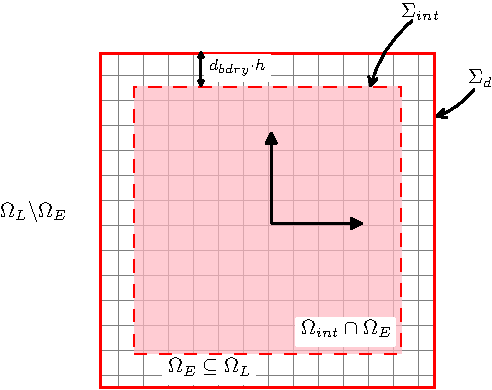
\includegraphics[width=0.5\linewidth]{./figures/hybrid/lambOseen/hlo_dd-crop.pdf}
	\caption{The domain decomposition for the Lamb-Oseen vortex problem, $\Omega_E \subseteq \Omega_L$. The Eulerian domain bounds $\Omega_E = [-0.5,0.5]\times[-0.5,0.5]$ with Dirichlet boundary $\partial \Omega_{dirichlet}$ [{\color{plotRed}{---}}, solid red] (\emph{not to scale}). The parameters of the discretization are tabulated in table \ref{tab:HLO_pt}.}
	\label{fig:HLO_dc}
	\end{figure}

Figure \ref{fig:HLO_dc} shows the Hybrid domain configuration for the Lamb-Oseen Vortex problem with the Lagrangian domain $\Omega_L$ spanning the full fluid domain. The Eulerian domain $\Omega_E$ only resolves the center of the Lamb-Oseen core, $\Omega_E \subseteq \Omega_L$. The domain bounds $[-0.5,-0.5] \times [-0.5,-0.5]$ with a Dirichlet velocity boundary $\Sigma_d$ where the velocity boundary condition is applied as described in section 
\ref{subsec:dbc}. The correction of the Lagrangian domain is performed in the interpolation domain $\Omega_{int}$ according to the procedures described in section \ref{sec:correction}. We that the interpolation domain $\Omega_{int}$ is offset from the Eulerian boundary $\Sigma_d$ by a distance $d_{bdry} = 2\cdot h$, where $h$ is the nominal blob spacing. Similar choice was made by Stock \cite{Stock2010a}, and ensures that the potential inaccuracies at the outer Eulerian boundary is ignored during the interpolation procedure.  

The spatial discretization of the Eulerian domain $\Omega_E$ is regarded as the control variable. Therefore, the parameter sensitivity analysis is performed by varying the spatial discretization of the Lagrangian method. The Eulerian domain is discretized with an unstructured mesh formulation using GMSH (see section \ref{subsec:mgugmsh}) having $N_{cells} = 26448$ unstructured cells and grid size $h_{grid}$ ranging from $0.007$ to $0.0016$. 

The Lamb-Oseen Vortex problem is defined according to the parameters tabulated in table \ref{tab:HLO_pt}. The core is located at $(0,0)$, where the Eulerian domain $\Omega_E$ is centered. The parameters are chosen such that vorticity $\omega$ and velocity $\mathbf{u}$ is non-zero at the boundary of the Eulerian domain $\Sigma_d$, figure \ref{fig:HLO_dc}. The Lamb-Oseen time constant $\tau = 100$ is chosen to ensure such vorticity distribution.

The evolution of the Lagrangian solver and the Eulerian solver is performed according to section \ref{sec:evolveLagrangian} and \ref{sec:evolveEulerian} respectively. The Lagrangian solver performs TRS for diffusion of the vortex blobs, see section \ref{subsubsec:srs}. The scheme requires vortex blob redistribution at every step, $f_{redis} = 1$. In conjunction with the redistribution, the population control is performed at every step, $f_{pc}=1$ with $(\Gamma_{loc},\Gamma_{glob})$ in table \ref{tab:HLO_pt}. 


\subsection{Results and Discussion}

The investigation of the Lamb-Oseen vortex problem is divided into three parts. The first part of the investigation concerns with comparing several stages of the hybrid coupling, section \ref{subsec:UvOvF}, where we compare the uncoupled scheme with the one-way coupled scheme and fully coupled scheme. These successive coupling investigate will help determine the source and quantify the error of the coupling. The second part of the investigation, section \ref{subsubsec:coc} focuses on importance of conservation of circulation that was discussed in section \ref{subsubsec:cc}. The results of the non-conserved and conserved scheme are compared to conclude the importance of conservation of circulation. During these two investigations, the parameters tabulated in table \ref{tab:HLO_pt} are used.

The third and final investigation is dedicated to the parameter sensitivity analysis, section \ref{subsubsec:psa}. Parameters that determine the spatial and temporal discretization of the scheme is investigated to verify the convergence of scheme.

\subsubsection{Uncoupled vs. One-way Coupled vs. Fully Coupled}
\label{subsec:UvOvF}
To verify the implementation of the hybrid algorithm, we compared several stages of the hybrid coupling with the standard, fully Eulerian test case. The three types of the coupling are as given:

\begin{itemize}
\item \textbf{Uncoupled}: The uncoupled test case involves only Eulerian solver and serves as a benchmark to quantify the error in coupling. The boundary conditions are determined directly from the analytical formulation, equation 	\ref{eq:eLO_veq}.
\item \textbf{One-way coupled}: The one-way coupled test case is a partially coupled hybrid test case where the Eulerian method is evolved using the Lagrangian solution. The correction of the Lagrangian solution is not performed in this scenario. Thus, this case will help us determine the error in evolution Eulerian method using the Lagrangian solution.
\item \textbf{Fully coupled}: The fully coupled test case performs the full coupling strategy described in section \ref{subsec:mcs}. The Eulerian method is evolved using the Lagrangian solution and the Lagrangian solution in the interpolation domain $\Omega_{int}$, figure \ref{fig:HLO_dc} is corrected at the end of each time step. This test case will help us quantify the error in transferring the Eulerian solution to the Lagrangian method.
\end{itemize}
	
	\begin{figure}[h]
     \centering
     \begin{subfigure}[t]{0.45\textwidth}
             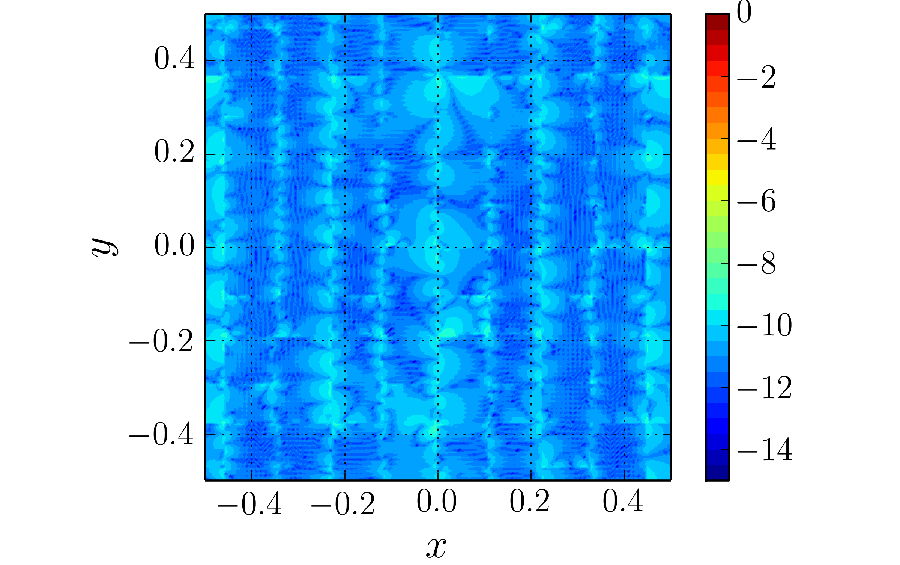
\includegraphics[width=\linewidth]{./figures/hybrid/lambOseen/lambOseen_fully_vErrorInitial_raster.pdf}
             \caption{Velocity}
             \label{fig:lambOseen_oneway_vErrorInitial}
     \end{subfigure}%
     \qquad %add desired spacing between images, e. g. ~, \quad, \qquad etc.
       %(or a blank line to force the subfigure onto a new line)
     \begin{subfigure}[t]{0.45\textwidth}
             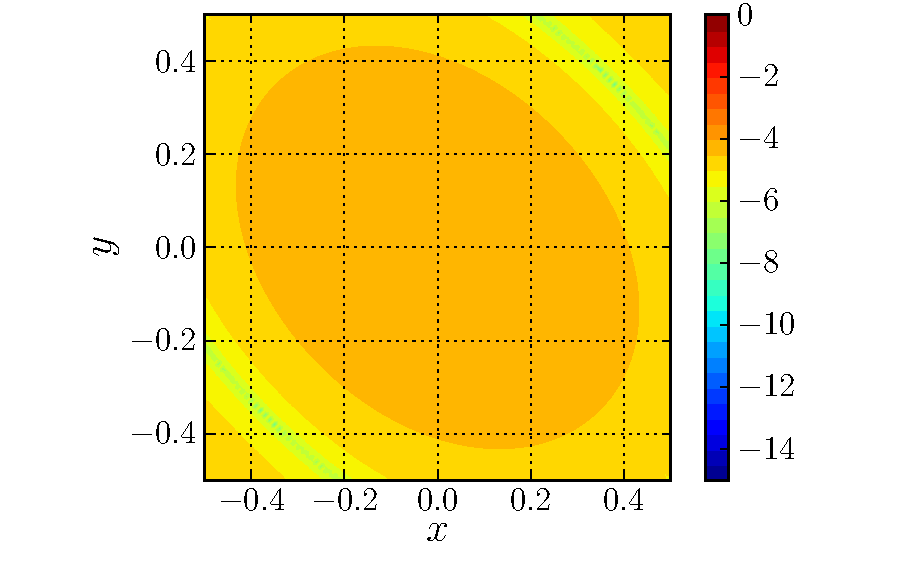
\includegraphics[width=\linewidth]{./figures/hybrid/lambOseen/lambOseen_fully_wErrorInitial_compressed.pdf}
             \caption{Vorticity}
             \label{fig:lambOseen_uncoupled_wErrorInitial}
     \end{subfigure}
     \caption{Initial relative error at $t=0$ inside the Eulerian domain. The figure depicts \textbf{(a)} the relative error in velocity $\mathbf{u}$ and \textbf{(b)} the relative error in vorticity $\omega$.}
     \label{fig:lambOseen_initialError}
	\end{figure}
		
Figure \ref{fig:lambOseen_initialError} depicts the initial relative error in velocity and vorticity inside the Eulerian domain $\Omega_E$. The relative error in velocity is near machine epsilon $\epsilon \le \num{e-8}$, but the error in vorticity is in the order \num{e-5}. Similar observation was made in section \ref{subsec:eulerianLambOseen} and arises from the projection error of the Finite Element when determining the vorticity $\omega$ from velocity $\mathbf{u}$, described in section \ref{subsec:dtvf}. 

	\begin{figure}[!t]
	\centering
	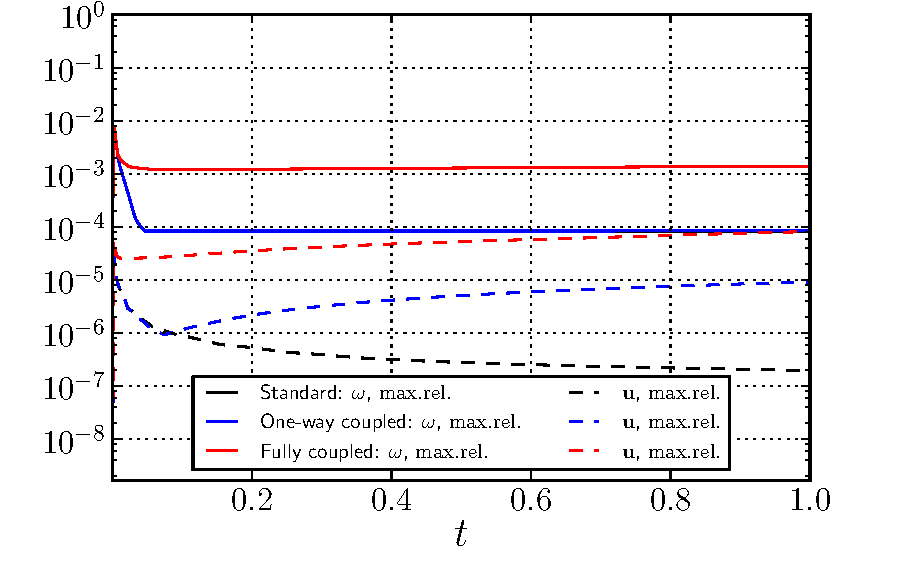
\includegraphics[width=0.6\linewidth]{./figures/hybrid/lambOseen/lambOseen_comparision_compressed.pdf}
	\caption{Comparison of the evolution of the maximum relative error in vorticity $\epsilon_{\omega}$ and maximum relative error in vorticity $\epsilon_{\mathbf{u}}$, equation \ref{eq:maxRelErrorDef}, from $t=0$ to $t=1$, using the parameters tabulated in table \ref{tab:HLO_pt}. The figure compares standard case (\textbf{black}) vs. the one-way coupled case ({\color{plotBlue}{\textbf{blue}}}) vs. the fully coupled case ({\color{plotRed}{\textbf{red}}}). The plot depicts maximum relative error in velocity (dashed), and the maximum relative error in vorticity (solid).}
	\label{fig:lambOseen_comparison}
	\end{figure}

The simulation was evolved from $t=0$ to $t=1$ with $N_{t-steps} = 1000$ Lagrangian and Eulerian time steps (i.e $k_E = 1$) using the time step parameters tabulated in table \ref{tab:HLO_pt}. Figure \ref{fig:lambOseen_comparison} shows the evolution of maximum relative error in vorticity $\omega$ and velocity $\mathbf{u}$ of the uncoupled, one-way coupled and the fully coupled cases in the Eulerian domain $\Omega_E$ w.r.t. the analytical solution, equation \ref{eq:lo_voeq}. The initial observation shows the error in velocity is two to three orders of magnitude less than the error in vorticity and occurs due to the projection error. The figure shows that the uncoupled scheme has the lowest error in vorticity and velocity. As the boundary condition is directly obtained from the analytical solution, the error only arises from FE discretization of the Eulerian method. As time progresses, the error in velocity $\epsilon_{\mathbf{u}}$ converges around \num{e-7} and the error in vorticity $\epsilon_{\omega}$ converges around \num{e-4}.

The one-way coupled case shows an increase in the error in velocity field inside the Eulerian domain $\Omega_E$. However, the difference is negligible in the initial stages of the simulation. This states that the discretization error of the analytical solution is also well represented by the vortex blobs. However by $t=1$, the error in velocity increases by two orders of magnitude from \num{e-7} to \num{e-5}. This implies that the error is due to the time integration error of the Lagrangian method. In section \ref{subsec:lagrangianLambOseen}, we observed similar trend and was caused by the growth in error due to time-marching of the vortex blobs.

	\begin{figure}[!p]
     \centering
     \begin{subfigure}[t]{0.45\textwidth}
             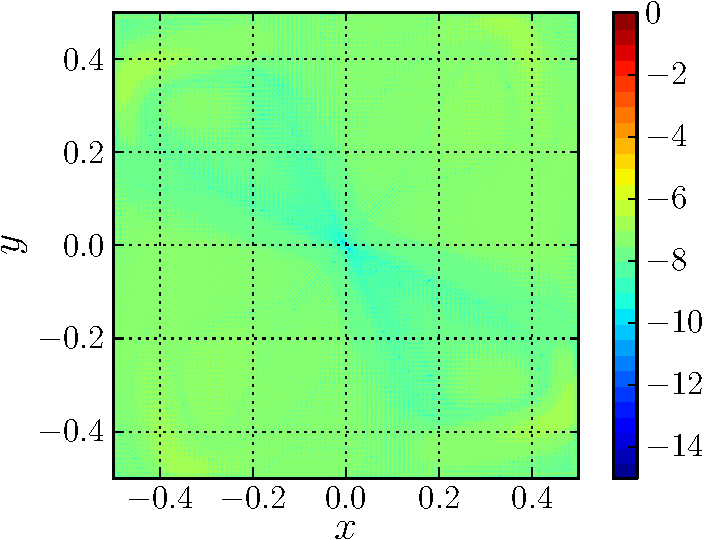
\includegraphics[width=\linewidth]{./figures/hybrid/lambOseent2/lambOseen_uncoupled_vErrorFinal_compressed-crop.pdf}
             \caption{Uncoupled; velocity $\mathbf{u}$}
             \label{fig:lambOseen_uncoupled_vErrorFinal}
     \end{subfigure}%
     \qquad %add desired spacing between images, e. g. ~, \quad, \qquad etc.
       %(or a blank line to force the subfigure onto a new line)
     \begin{subfigure}[t]{0.45\textwidth}
             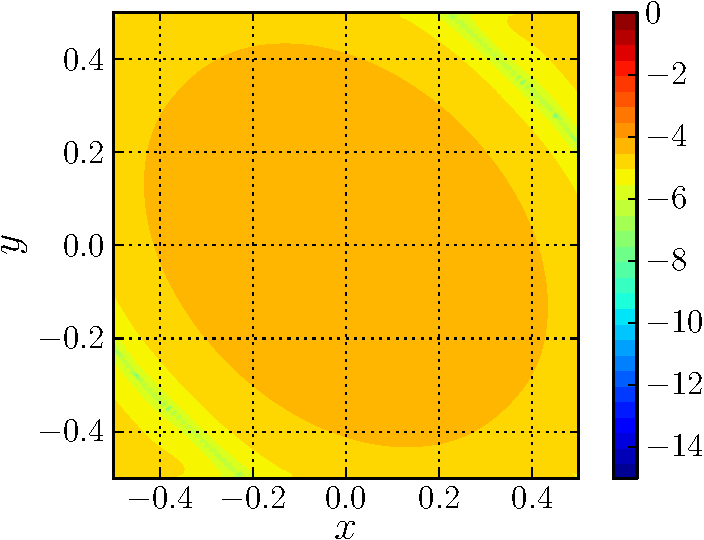
\includegraphics[width=\linewidth]{./figures/hybrid/lambOseent2/lambOseen_uncoupled_wErrorFinal_compressed-crop.pdf}
             \caption{Uncoupled; vorticity $\omega$}
             \label{fig:lambOseen_uncoupled_wErrorFinal}
     \end{subfigure}%       
       
     \begin{subfigure}[t]{0.45\textwidth}
             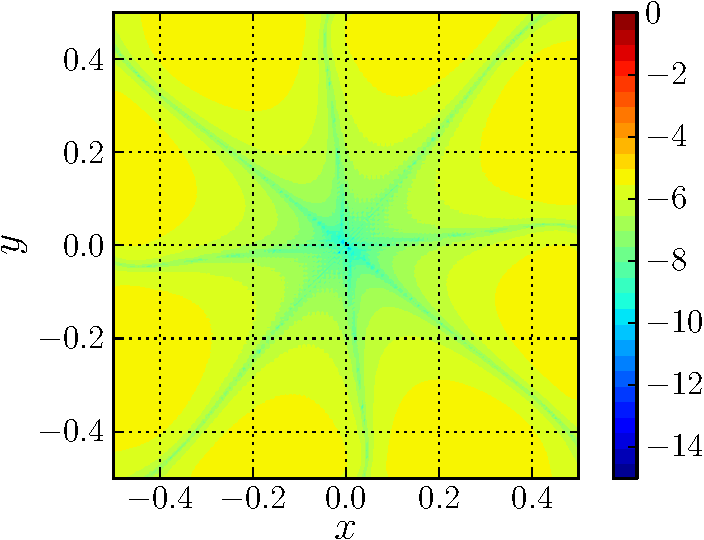
\includegraphics[width=\linewidth]{./figures/hybrid/lambOseent2/lambOseen_oneway_vErrorFinal_compressed-crop.pdf}
             \caption{One-way coupled; velocity $\mathbf{u}$}
             \label{fig:lambOseen_oneway_vErrorFinal}
     \end{subfigure}
     \qquad
     \begin{subfigure}[t]{0.45\textwidth}
             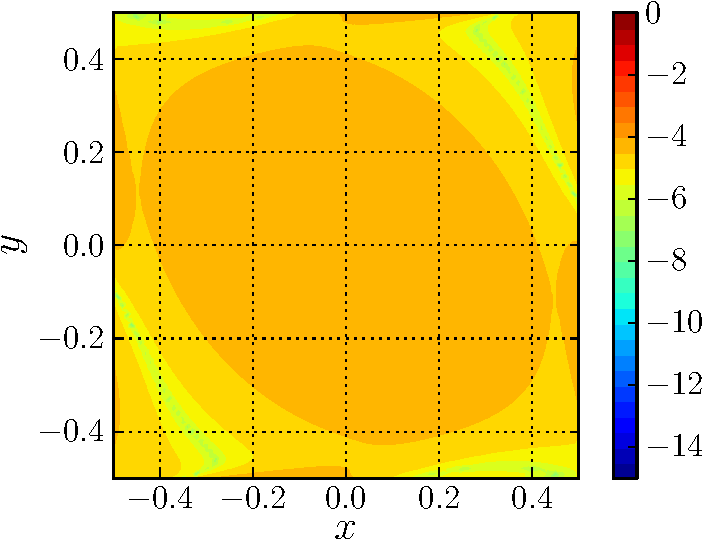
\includegraphics[width=\linewidth]{./figures/hybrid/lambOseent2/lambOseen_oneway_wErrorFinal_compressed-crop.pdf}
             \caption{One-way coupled; vorticity $\omega$}
             \label{fig:lambOseen_oneway_wErrorFinal}
     \end{subfigure}     
   
     \begin{subfigure}[t]{0.45\textwidth}
             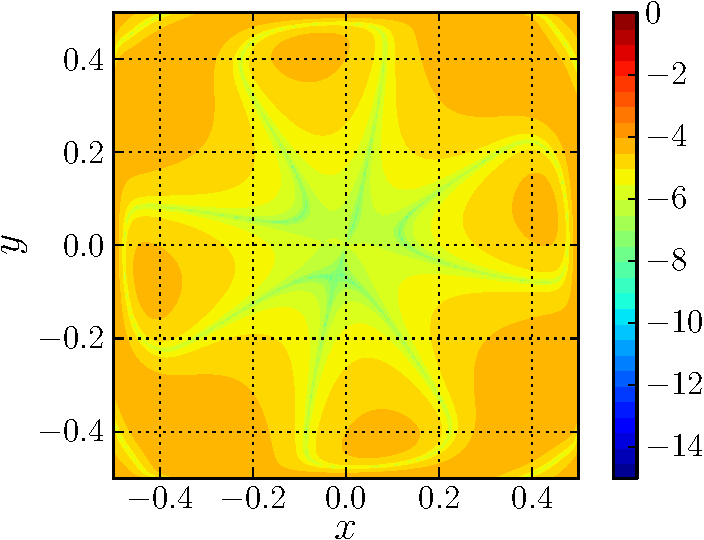
\includegraphics[width=\linewidth]{./figures/hybrid/lambOseent2/lambOseen_fully_vErrorFinal_compressed-crop.pdf}
             \caption{Fully coupled; velocity $\mathbf{u}$}
             \label{fig:lambOseen_fully_vErrorFinal}
     \end{subfigure}     
     \qquad
     \begin{subfigure}[t]{0.45\textwidth}
             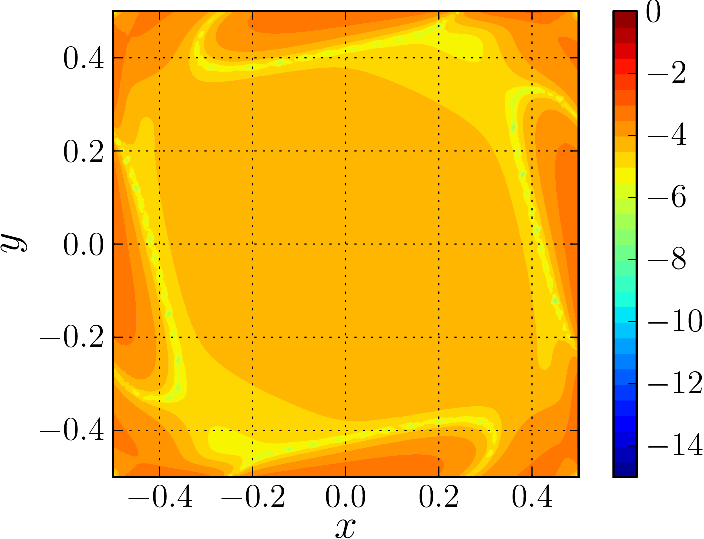
\includegraphics[width=\linewidth]{./figures/hybrid/lambOseent2/lambOseen_fully_wErrorFinal_compressed-crop.pdf}
             \caption{Fully coupled; vorticity $\omega$}
             \label{fig:lambOseen_fully_wErrorFinal}
     \end{subfigure}        
     
     \caption{Plot of the relative error in velocity (\textit{left}) and relative error in vorticity (\textit{right}) in the Eulerian domain $\Omega_E$ at $t=1$. The figure compares the error between \textbf{(a)},\textbf{(b)} the uncoupled, \textbf{(c)},\textbf{(d)} the one-way coupled and \textbf{(e)},\textbf{(f)} the fully coupled cases.}
     \label{fig:lambOseen_finalError}
	\end{figure}

The fully coupled case demonstrates that there is an additional increase in the error. Unlike the one-way coupled case, the increase in the error is observed from the initial stages. This implies that the increasing in error is solely due to the transfer of vorticity from the Eulerian method to the Lagrangian method. A transfer of the discrete vorticity field from the Eulerian method to the Lagrangian method causes an additional increase in error of the Lagrangian solution, deviating the Lagrangian solution further from the analytical solution. Furthermore, in section \ref{subsec:hy_iwtca}, we discussed that the Gaussian blurring of the vorticity field adds an additional error when re-initializing the vortex blobs inside the interpolation domain $\Omega_{int}$. The consequence of this is that at $t=1$, the error in vorticity $\epsilon_{\omega}$ increased from \num{e-4} to \num{e-3} and the error in velocity $\epsilon_{\mathbf{u}}$ increased from \num{e-5} to \num{e-4}.
	
Figure \ref{fig:lambOseen_finalError} shows the relative error in velocity and vorticity inside the Eulerian domain $\Omega_E$ at $t=1$, for the three types of coupling. We observe that the error increases as one moves from uncoupled to one-way coupled and one-way coupled to fully coupled. As one goes from uncoupled to one-way coupled, the increase in the error is observed at the boundaries. This implies that the error originates from error in the Dirichlet boundary conditions at the boundary $\Sigma_d$. Comparing the one-way coupled to fully coupled case, we see that the boundary generates additional error. Figure \ref{fig:lambOseen_fully_wErrorFinal} clearly shows this artificial vorticity generated from the boundary due to the mismatch in the solutions of the Eulerian and the Lagrangian method. 

The strength of the artificial vorticity at the boundary is proportional to the error in the coupling and to ensure an accurate coupling scheme, we have ensure this vorticity does not corrupt the solution. Therefore, to ensure this, we have to modify the discretization such that this vorticity is less the threshold of influence (i.e $<1\%$ of the maximum vorticity $\max\{\omega\}$).

\subsubsection{Conservation of circulation}
\label{subsubsec:coc}

The approach for ensuring conservation of circulation during the coupling was discussed in section \ref{subsubsec:cc}. To validate the importance of conservation of circulation, we ran two simulation with and without the conservation of circulation during the transfer of vorticity from the Eulerian method to the Lagrangian method. All the other parameters of the simulation were maintained according to table \ref{tab:HLO_pt}.

Figure \ref{fig:lambOseen_conservation_contourf} compares the error in the Eulerian domain $\Omega_E$ at $t=1$ of the coupling approach without conservation circulation against the approach satisfying the conservation of circulation. We see that the scheme without conservation has significantly larger error in the domain than the with conservation. The maximum error is near the Dirichlet boundary $\Sigma_d$ and shows artificial vorticity emanating from the boundary due to this larger mismatch in the solutions, figure \ref{fig:lambOseen_fullyCoff_wErrorFinal}. However, when we ensure that circulation is conserved, figure \ref{fig:lambOseen_fullyCon_wErrorFinal}, the boundary produces significantly less error.

	\begin{figure}[!p]
     \centering
     \begin{subfigure}[t]{0.45\textwidth}
             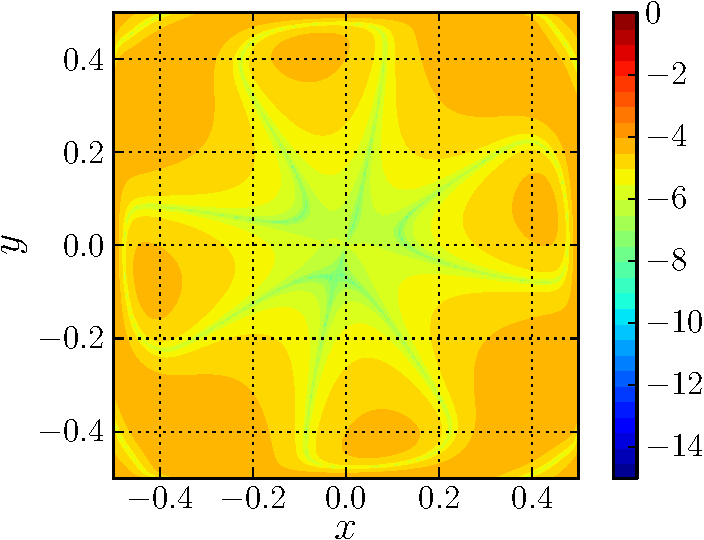
\includegraphics[width=\linewidth]{./figures/hybrid/lambOseent2/lambOseen_fully_vErrorFinal_compressed-crop.pdf}
             \caption{Conservation \texttt{on}; velocity $\mathbf{u}$}
             \label{fig:lambOseen_fullyCon_vErrorFinal}
     \end{subfigure}%
     \qquad %add desired spacing between images, e. g. ~, \quad, \qquad etc.
       %(or a blank line to force the subfigure onto a new line)
    \begin{subfigure}[t]{0.45\textwidth}
             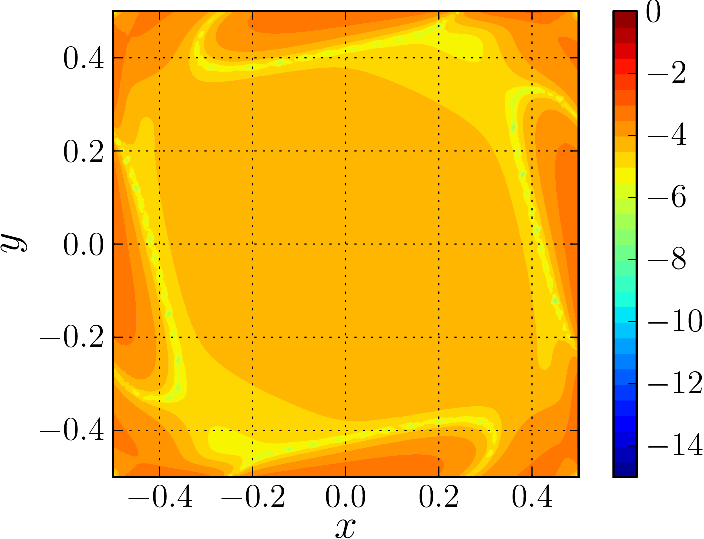
\includegraphics[width=\linewidth]{./figures/hybrid/lambOseent2/lambOseen_fully_wErrorFinal_compressed-crop.pdf}
             \caption{Conservation \texttt{on}; vorticity $\omega$}
             \label{fig:lambOseen_fullyCon_wErrorFinal}
     \end{subfigure}%     
            
     \begin{subfigure}[t]{0.45\textwidth}
             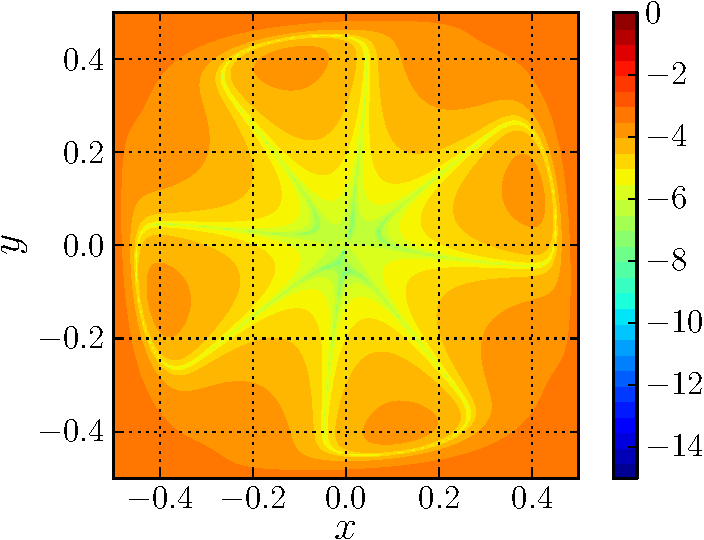
\includegraphics[width=\linewidth]{./figures/hybrid/lambOseent2/lambOseen_fullyCoff_vErrorFinal_compressed-crop.pdf}
             \caption{Conservation \texttt{off}; velocity $\mathbf{u}$}
             \label{fig:lambOseen_fullyCoff_vErrorFinal}
     \end{subfigure}
     \qquad     
     \begin{subfigure}[t]{0.45\textwidth}
             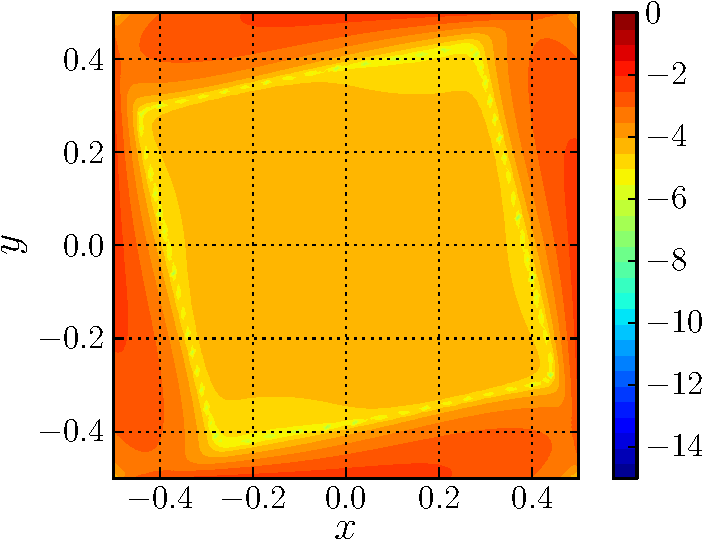
\includegraphics[width=\linewidth]{./figures/hybrid/lambOseent2/lambOseen_fullyCoff_wErrorFinal_compressed-crop.pdf}
             \caption{Conservation \texttt{off}; vorticity $\omega$}
             \label{fig:lambOseen_fullyCoff_wErrorFinal}
     \end{subfigure}  
  
     \caption{Plot of the relative error in velocity (left) and the relative error in vorticity (right) in the Eulerian domain $\Omega_E$ at $t=1$. The figure compares the error between \textbf{(a)}\textbf{(b)} without conservation of circulation, and \textbf{(c)}\textbf{(d)} with the conservation of circulation.}
     \label{fig:lambOseen_conservation_contourf}
	\end{figure}
	
	\begin{figure}[!p]
	\centering
	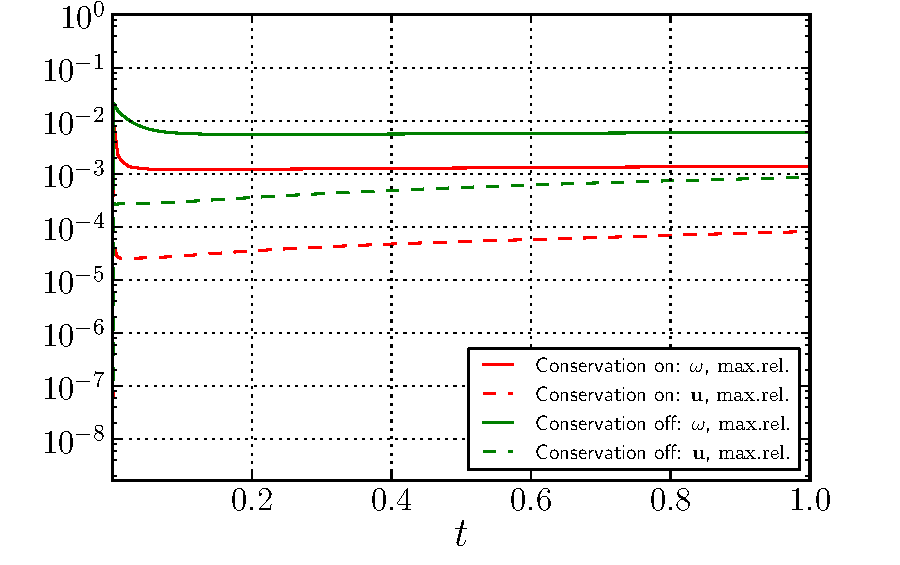
\includegraphics[width=0.6\linewidth]{./figures/hybrid/lambOseent2/lambOseen_comparision_conservation_compressed.pdf}
	\caption{Plot of the maximum relative error in vorticity $\epsilon_{\omega}$ [ - -, dashed] and maximum relative error in vorticity $\epsilon_{\mathbf{u}}$ [ ---, solid], equation \ref{eq:maxRelErrorDef}, from $t=0$ to $t=1$, using the parameters tabulated in table \ref{tab:HLO_pt}. The figure compares the coupling scheme with conservation of circulation ({\color{plotRed}{\textbf{red}}}) vs. the coupling scheme without conservation of circulation ({\color{plotGreen}{\textbf{green}}}).}
	\label{fig:lambOseen_comparision_conservation}
	\end{figure}	

Figure \ref{fig:lambOseen_comparision_conservation} shows the evolution of the maximum relative error from $t=0$ to $t=1$, comparing the results of with conservation and without conservation of circulation. Observing the difference in the error in velocity and the error in vorticity, we see that the scheme without conservation produces larger error at all times. At $t=1$, we observe that scheme without conservation has error in vorticity near \num{e-2}, whereas with conservation, the error is an order of magnitude lower at \num{e-3}. Similarly for velocity, for the scheme without conservation the error approaches \num{e-3}, whereas with conservation, the error only reaches \num{e-4}. 

Figure \ref{fig:lambOseen_comparision_conservation_circulation} shows the change in total circulation from $t=0$ to $t=1$ for the non-conserved and conserved scheme. It is apparent that without the conservation of circulation, the error in total circulation significantly larger and approaches \num{e-3}. As the circulation is not conserved explicitly, the transfer of vorticity from the Eulerian method to the Lagrangian method introduces error in total circulation. By ensuring conservation of circulation, section \ref{subsubsec:cc}, we see that the error in total circulation is near \num{e-10}. It is to be noted that the linear increase in the error in total circulation is due to the population control of the vortex blobs, removing the circulation $\Gamma_{glob}$ at every evaluation, as described in section \ref{subsubsec:srs}.

	\begin{figure}[!h]
	\centering
	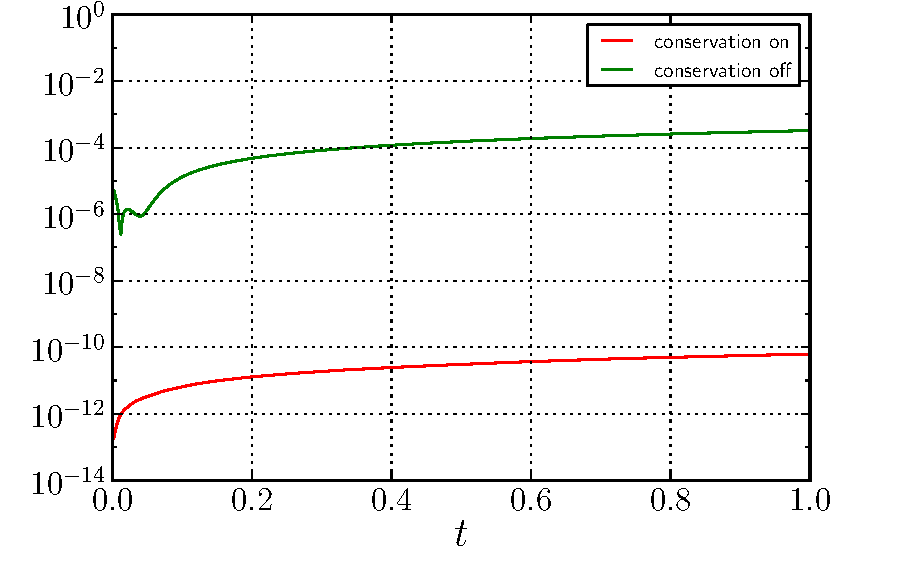
\includegraphics[width=0.6\linewidth]{./figures/hybrid/lambOseent2/lambOseen_comparision_conservation_circulation_compressed.pdf}
	\caption{Plot of the error in total circulation $\epsilon_{\Gamma}$ of the Lagrangian method from $t=0$ to $t=1$. The figure compares the scheme with conservation of circulation [ {\color{plotRed}{\textbf{---}}}, solid {\color{plotRed}{\textbf{red}}}], and the scheme without conservation of circulation [ {\color{plotGreen}{\textbf{---}}}, solid {\color{plotGreen}{\textbf{green}}}].}
	\label{fig:lambOseen_comparision_conservation_circulation}
	\end{figure}	

In summary, we have determined that to ensure minimum error during the transfer of Eulerian solution to the Lagrangian solution, we have to ensure that circulation is conserved.

\subsubsection{Parameter sensitivity analysis}
\label{subsubsec:psa}

The parameter sensitivity analysis is the last stage of the Lamb-Oseen vortex investigation. The Lamb-Oseen vortex test case is ideal to determine the effects of temporal and spatial discretization on the accuracy of the coupling. 

To investigate the effects of the spatial discretization on the accuracy of the coupling, we ran several test cases varying the nominal blob spacing $h$, and test cases varying the overlap ratio $\lambda$. To investigate the effects of temporal discretization, we modified the Lagrangian time step size $\Delta t_L$ w.r.t the Eulerian time step size $\Delta t_E$. The control variables of the simulations were chosen to be that of the previous simulations, as tabulated in table \ref{tab:HLO_pt}.

	\begin{figure}[!h]
	\centering
	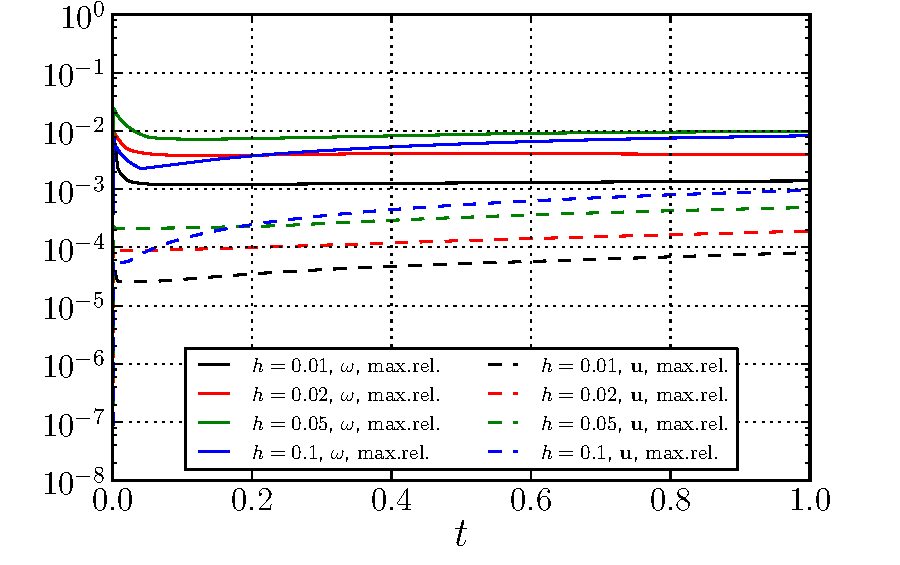
\includegraphics[width=0.6\linewidth]{./figures/hybrid/lambOseen/lambOseen_parameter_h.pdf}
	\caption{Comparison the evolution of error for various nominal blob spacing $h = [0.01,0.02,0.05,0.1]$. The figures shows the maximum relative error in vorticity $\epsilon_{\omega}$ [ - -, dashed] and maximum relative error in vorticity $\epsilon_{\mathbf{u}}$ [ ---, solid], equation \ref{eq:maxRelErrorDef}, from $t=0$ to $t=1$, with control variables from table \ref{tab:HLO_pt}.}
	\label{fig:lambOseen_parameter_h}
	\end{figure}	
	
Figure \ref{fig:lambOseen_parameter_h} shows the impact of varying the nominal blob spacing $h$ on the coupling. The maximum relative error in vorticity $\epsilon_{\omega}$ and the maximum relative error in velocity $\epsilon_{\mathbf{u}}$ is plotted from $t=0$ to $t=1$ for nominal blob spacing $h = [0.01,0.02,0.05,0.1]$. The figure shows that the reducing the spatial resolution of the Lagrangian method increases the error. At $t=1$, the minimum error is observed for $h=0.01$ with the error in velocity at \num{e-4} and the error in vorticity at \num{e-3}, at $t=1$. The maximum error is observed for $h=0.1$, increasing to \num{e-3} for the error in velocity and to \num{e-2} for the error in vorticity. This implies that the growth in error is order 1. Figure \ref{fig:lambOseen_parameter_h_Trend} shows the variation in error in vorticity at $t=1$ for various $h$. The figure agrees with our previous observation, and shows change in error in coupling due to the spatial discretization is of order one.

	\begin{figure}[!h]
	\centering
	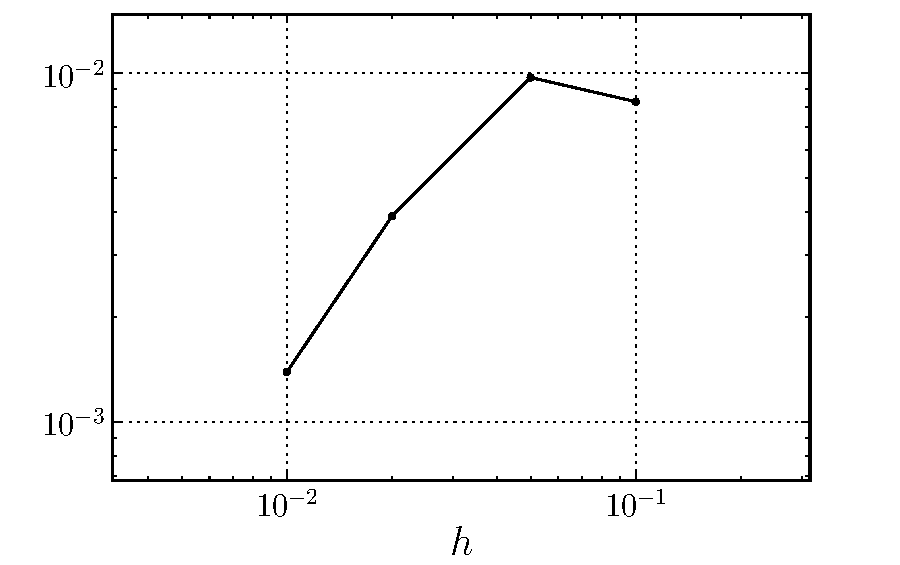
\includegraphics[width=0.6\linewidth]{./figures/hybrid/lambOseen/lambOseen_parameter_h_Trend.pdf}
	\caption{Convergence of the error in coupling due to the nominal blob spacing $h$. The control variables are tabulated in table \ref{tab:HLO_pt}.}
	\label{fig:lambOseen_parameter_h_Trend}
	\end{figure}	

Figure \ref{fig:lambOseen_parameter_overlap} compares the evolution of the error for various overlap ratios, $\lambda = [0.5, 0.75, 1.0, 1.5]$. We see that the minimum error in velocity and vorticity is observed for the overlap ratio $\lambda = 1$. As we vary from this value, an increase in error is observable. In section \ref{subsubsec:convergenceInterpolation}, we determined that to reduce the Gaussian blurring of the vorticity field due to the vortex blobs, we require an overlap ratio near $\lambda=1$ and a reduction in nominal blob spacing $h$. The parameter sensitivity analysis on the spatial discretization validates this observation and states that to ensure minimum error in coupling, these criteria has to be satisfied.

	\begin{figure}[!h]
	\centering
	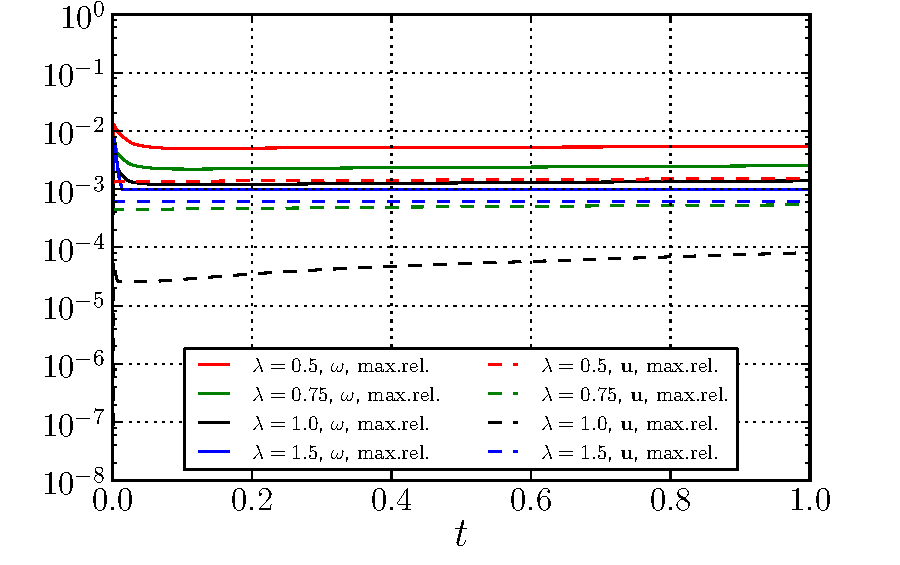
\includegraphics[width=0.6\linewidth]{./figures/hybrid/lambOseen/lambOseen_parameter_overlap.pdf}
	\caption{Comparison the evolution of error for various overlap ratios $\lambda = [0.5, 0.75, 1.0, 1.5]$. The figures shows the maximum relative error in vorticity $\epsilon_{\omega}$ [ - -, dashed] and maximum relative error in vorticity $\epsilon_{\mathbf{u}}$ [ ---, solid], equation \ref{eq:maxRelErrorDef}, from $t=0$ to $t=1$, with control variables from table \ref{tab:HLO_pt}.}
	\label{fig:lambOseen_parameter_overlap}
	\end{figure}	

Figure \ref{fig:lambOseen_parameter_k} shows the varying the temporal discretization of the Lagrangian method and the Eulerian method w.r.t each other. The relation of the Eulerian time step size $\Delta t_E$ to the Lagrangian time step size $\Delta t_L$ is described in section \ref{subsec:mse}. Figure \ref{fig:lambOseen_parameter_k_dtL} shows the effect of modifying the Lagrangian time step size $\Delta t_L$ w.r.t to the Eulerian time step size $\Delta t_E=0.001$, with $\Delta t_L = k_E\cdot\Delta t_E$ for $\Delta t_E = 0.001$ and the number of Eulerian sub-steps $k_E = [1,2,5,10]$. Similarly, figure \ref{fig:lambOseen_parameter_k_dtE} shows the effect of modifying the Eulerian time step size $\Delta t_E$ w.r.t to the Lagrangian time step, with $\Delta t_E = \Delta t_L/k_E$ for $\Delta t_L=0.001$ and $k_E = [1,2,5]$. We see that the minimum error occurs when the time steps match, $\Delta t_L = \Delta t_E$. However if increase the number of Eulerian time steps from $k_E = 1 $ to $k_E=2$, there an substantial increase in the error in velocity. Whereas, increasing $k_E=2$ to $k_E=5$, only increases the error slightly. This observation states that the linear interpolation used for sub-stepping process, has potential for improvement. A possible solution might be to employ a higher-order interpolation method for determining the Eulerian Dirichlet boundary condition at the sub-steps.

	\begin{figure}[!h]
     \centering
     \begin{subfigure}[t]{0.45\textwidth}
             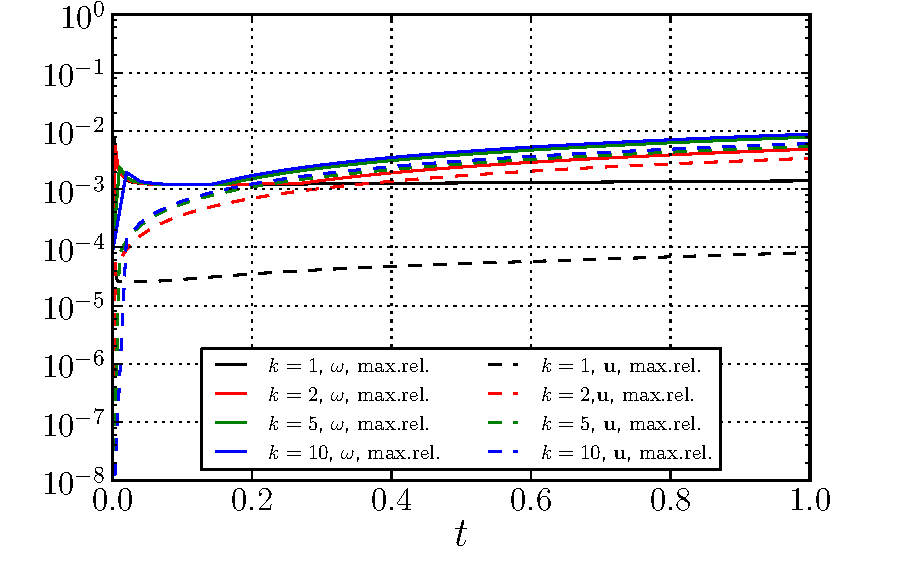
\includegraphics[width=\linewidth]{./figures/hybrid/lambOseen/lambOseen_parameter_k.pdf}
             \caption{$\Delta t_L = [0.001,0.002,0.005,0.01]$, $\Delta t_E = 0.001$}
             \label{fig:lambOseen_parameter_k_dtL}
     \end{subfigure}     
     \qquad
     \begin{subfigure}[t]{0.45\textwidth}
             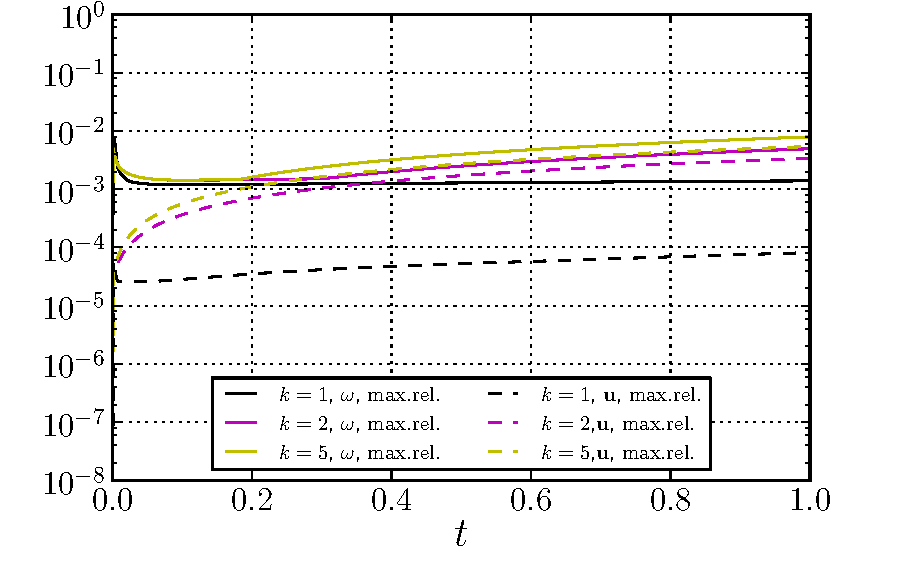
\includegraphics[width=\linewidth]{./figures/hybrid/lambOseen/lambOseen_parameter_k_dtE.pdf}
             \caption{$\Delta t_E = [0.001,0.0005,0.0002]$, $\Delta t_L = 0.001$}
             \label{fig:lambOseen_parameter_k_dtE}
     \end{subfigure}        
     
     \caption{Comparison the evolution of error for various number of Eulerian sub-steps $k_E = [1,2,5,10]$, by modifying the Lagrangian time step size $\Delta t_L$ and Eulerian time step size $\Delta t_E$. The figures shows the maximum relative error in vorticity $\epsilon_{\omega}$ [ - -, dashed] and maximum relative error in vorticity $\epsilon_{\mathbf{u}}$ [ ---, solid], equation \ref{eq:maxRelErrorDef}, from $t=0$ to $t=1$, with control variables of table \ref{tab:HLO_pt}.}
     \label{fig:lambOseen_parameter_k}
	\end{figure}	

%Figure \ref{fig:lambOseen_parameter_k_Trend} shows the convergence trend of error in vorticity due to number of Eulerian sub-step $k_E$. 
%
%	\begin{figure}[!h]
%	\centering
%	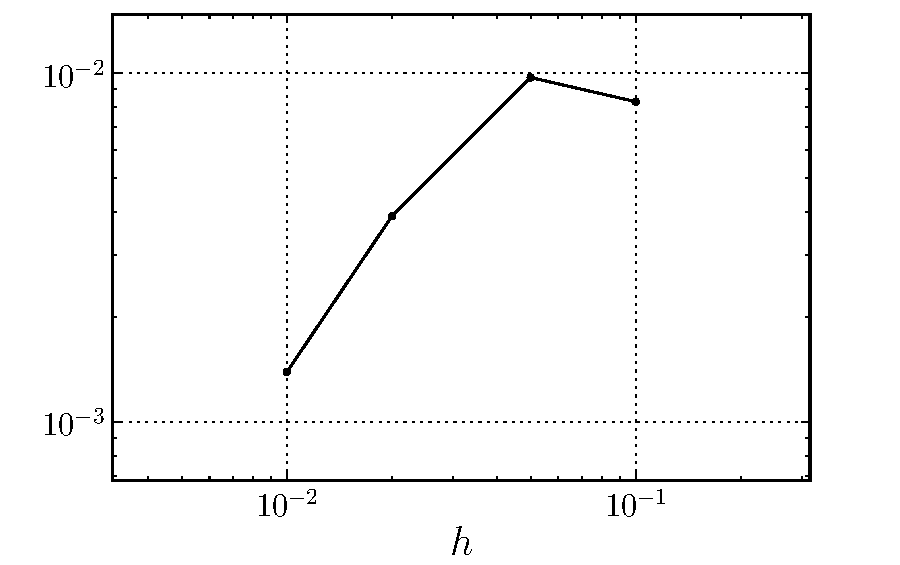
\includegraphics[width=0.6\linewidth]{./figures/hybrid/lambOseen/lambOseen_parameter_h_Trend.pdf}
%	\caption{Convergence of the error in coupling due to the number of Eulerian sub-step $k_E$ at $t=1$. The control variables are tabulated in table \ref{tab:HLO_pt}}.
%	\label{fig:lambOseen_parameter_k_Trend}
%	\end{figure}

\subsection{Conclusion}

In section \ref{}, we observed that moving from uncoupled to one-way coupled case increase the error in velocity. When moving from one-way coupled to fully coupled, there is an increase in error in vorticity and an additional increase in error in velocity.

In section \ref{}, we observed that conservation of circulation is vital in ensure an accurate coupling strategy. The transfer of vorticity from the Eulerian method to the Lagrangian method does not explicitly ensure conservation of circulation and introduces artificial vorticity from the Eulerian Dirichlet boundary $\Sigma_d$, figure .

In section \ref{}, we investigated the impact of varying the spatial and temporal discretization on the accuracy of the coupling. We determined there is an increase in error, if the Lagrangian method is spatially under-resolved w.r.t to the Eulerian method. An overlap ration $\lambda=1$ was shown to have the minimum error during the coupling, as it ensures minimum Gaussian blurring. Varying the number of Eulerian sub-steps $k_E$, showed that the linear interpolation for the Dirichlet boundary condition requires improvement in future.


\section{Clercx-Bruneau Dipole Convection}

In section ref{}, we determine the effects of transferring the Lagrangian solution to the Eulerian method, and transferring the Eulerian solution back to the Lagrangian method using an expanding vortex core (Lamb-Oseen vortex). However, an important aspect of domain decomposition method is the entry and the exist of a vortex core in the Eulerian domain $\Omega_E$. Tho investigate this aspect, we employed the Clercx-Bruneau dipole \cite{} convecting through a finite Eulerian domain. 

\subsection{Problem Definition}

The hybrid domain decomposition of the this investigation is depicted in figure \ref. The Eulerian domain $\Omega_E$ is finite with bounds $[-0.25,0.25]\times[-0.5,0.5]$ and is a subset of the Lagrangian domain $\Omega_L$, $\Omega_E \subseteq \Omega_L$. The Clercx-Bruneau dipole, equation \ref{fig:hcbconv_dd}, is initialized outside the Eulerian domain $\Omega_L\backslash\Omega_E$ at $(x_1,y_1) = (-1,0.1)$ and $(x_2,y_2)=(-1,-0.1)$, corresponding to the positive and negative core respectively. As the simulation progresses, the dipole convects along the $x$-axis, passing through the Eulerian domain.

	\begin{figure}[!p]
	\showthe\columnwidth
	\centering
	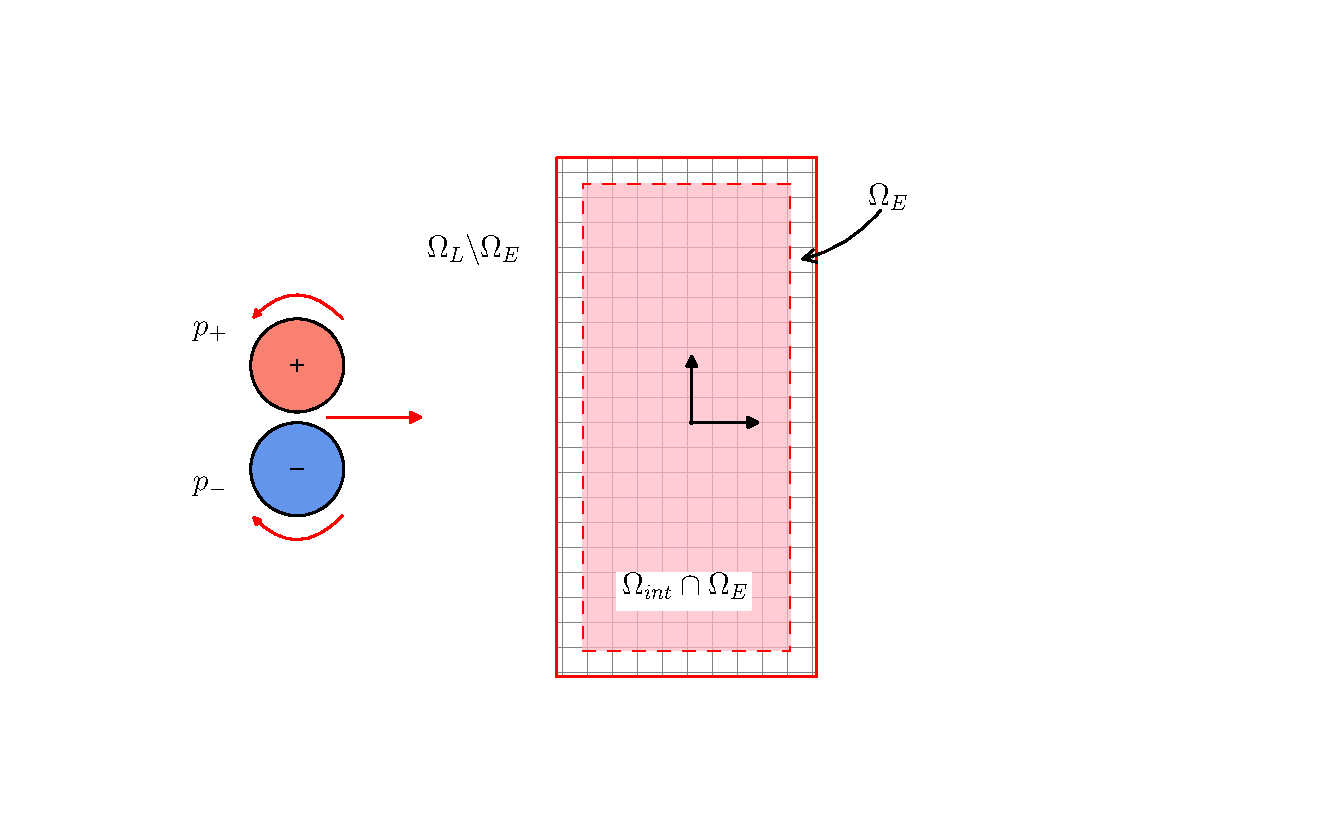
\includegraphics[trim=0cm 2.5cm 0cm 2.5cm, clip, width=\linewidth]{./figures/hybrid/cbConv/hcbconv_dd.pdf}
	\caption{[\textit{Not to Scale}] The domain decomposition for the Clercx-Bruneau convection problem, $\Omega_E \subseteq \Omega_L$, with the positive pole at $p_{+}=(x_1,y_1) = (-1,0.1)$ and negative pole at $p_{-}=(x_2,y_2)=(-1,-0.1)$. The parameters of the simulation are tabulated in table \ref{tab:HcbConvection_pt}.}
	\label{fig:hcbconv_dd}
	\end{figure}
	
The Eulerian and the Lagrangian domain is discretized according to the parameters shown in table \ref{tab:HcbConvection_pt}. The focus of this simulation is entry and the exist of vorticity from the Eulerian domain and it's impact on the solution. The simulation was first ran for a Finite Element only method (FE), and a Vortex Particle Method (VPM) only simulation. The purpose of these simulation was to sever as a benchmark for the hybrid study. To ensure that FE only simulation was valid, the Eulerian domain $\Omega_E$ stretched up to the far-field of the dipole, where its vorticity and the induced velocity was zero. The Eulerian domain $\Omega_E$ of the FE only simulation spanned $[-3,3]\times[-2,2]$. For a valid comparison, theses simulation followed the parameters tabulated in table \ref{tab:HcbConvection_pt} as well.

	\ctable[
		caption = {Summary of the parameters for the Clercx-Bruneau dipole convection problem.},
		label   = {tab:HcbConvection_pt},
		pos = !p,]{lcll}{}{\FL
		
		Parameters 					& Value 	& Unit					& Description \ML
		$\Omega_E$             		& $[-0.25,0.25]\times[-0.5,0.5]$ &\si{m}	& Eulerian domain bounds \\
		$Re$						& 625 & - & Reynolds number\\
		$U$							& 1 & \si{m.s^{-1}} & Characteristic velocity\\
		$W$							& 1 & \si{m} & Characteristic Length\\
		$\nu$						& \num{1.6e-3} & \si{kg.s^{-1}.m^{-1}} & Kinematic viscosity\\
		$(x,y)_{1,2}$				& $(-1,\pm0.1)$ & \si{m} & Initial location of the monopoles\\
		$\omega_e$					& 299.528385375226 & - & Characteristic vorticity of the monopole \cite{Renac2013}\\
		$\lambda$					& 1 & - & Overlap ratio\\
		$h$							& 0.005 & \si{m} & Nominal blob spacing\\
		$h_{grid}$ 					& $\approx0.007$ & \si{m}	& FE cell diameter \\
		$ N_{\mathrm{cells}}$ 		& $40000$ 	& -						& Number of mesh cells\\
		$\Delta t_L$				& \num{2.5e-4} & \si{s} & Lagrangian time step size\\
		$\Delta t_E$				& \num{2.5e-5} & \si{s} & Eulerian time step size\\		
		$k_E$						& 10 & - & Eulerian sub-steps\\
		$ N_{\mathrm{t-steps}}$ 	& 2800 & -			& Number of time integration steps\\
		$t$							& 0 to 0.7 & - & Simulation time\\
		$d_{bdry}$					& $2\cdot{h}$ & \si{m} & Interpolation boundary offset\LL}


\subsection{Results and Discussion}

	\begin{figure}[!b]
	\showthe\columnwidth
	\centering
	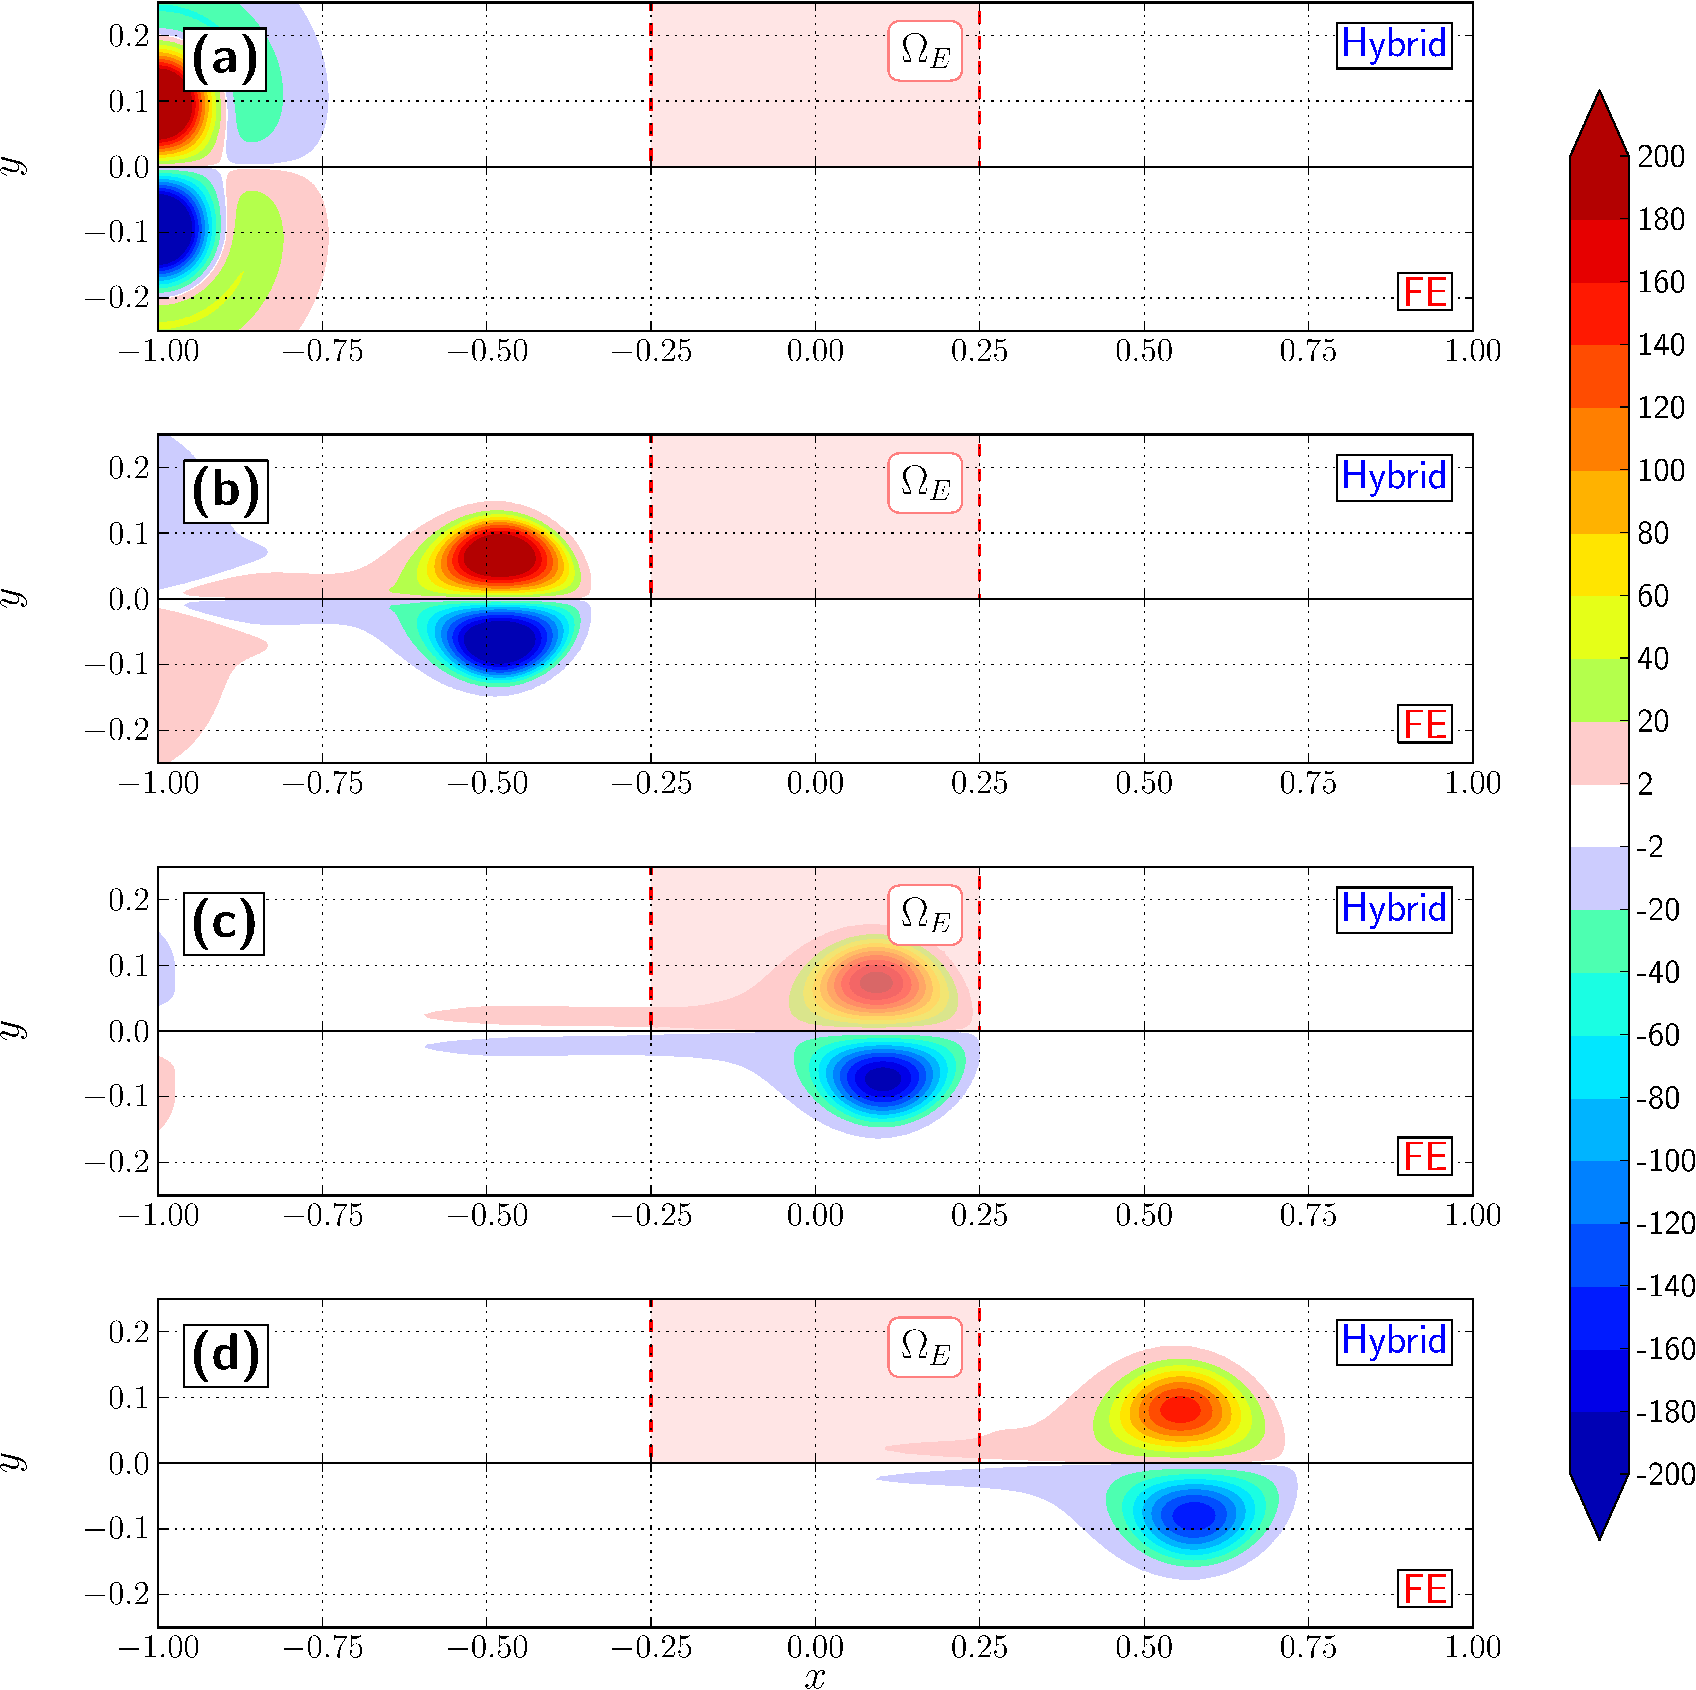
\includegraphics[width=\linewidth]{./figures/hybrid/cbConv/hybrid_doubleMonopoleConvection_contourfPlots-crop_compressed.pdf}
	\caption{Plot of the Clercx-Bruneau dipole at $t=[0,0.2,0.4,0.7]$ using parameters tabulated in table \ref{}. The figure compares the hybrid simulation (top halves) against the FE only simulation (bottom halves).}
	\label{fig:hybrid_doubleMonopoleConvection_contourfPlots}
	\end{figure}

Figure \ref{fig:hybrid_doubleMonopoleConvection_contourfPlots} compares the state of the dipole of the FE simulation and the hybrid simulation at times $t=[0,0.2,0.4,0.6]$. The top half of each subplot belongs to the hybrid simulation, whereas the bottom half to the FE only simulation. It was determined that the peak vorticity of the dipole enters the Eulerian domain $\Omega_E$ at $t=0.26$ and exits at $t=0.45$. The figure shows that solution of both simulation matches up to the entry of the dipole, figure \ref{fig:hybrid_doubleMonopoleConvection_contourfPlots}a and figure Figure \ref{fig:hybrid_doubleMonopoleConvection_contourfPlots}b. However in figure \ref{fig:hybrid_doubleMonopoleConvection_contourfPlots}c, the solutions start to become different, and at $t=0.7$, figure \ref{fig:hybrid_doubleMonopoleConvection_contourfPlots}d, it is apparent that the dipole in the hybrid method is lagging w.r.t to the FE only simulation. This would imply that the passage of the vortex through the domain has a stalling influence on the vorticity evolution.

To investigate further on this influence of the passage, we analyzed variation in maximum vorticity $\omega_{max}$. Figure \ref{fig:hybrid_dipoleConvection_hybridSubDomains_wMax} shows evolution of the maximum vorticity $\omega_{max}$ from $t=0$ to $t=0.7$ in the Eulerian domain $\Omega_E$ of the hybrid simulation, the Lagrangian domain $\Omega_L$ of the hybrid simulation, the FE only simulation, and the VPM only simulation. We observe there is a slight difference in the maximum vorticity for the FE only and the VPM only simulation and the difference increase as the time progresses. 

	\begin{figure}[!h]
     \centering
     \begin{subfigure}[t]{0.48\textwidth}
             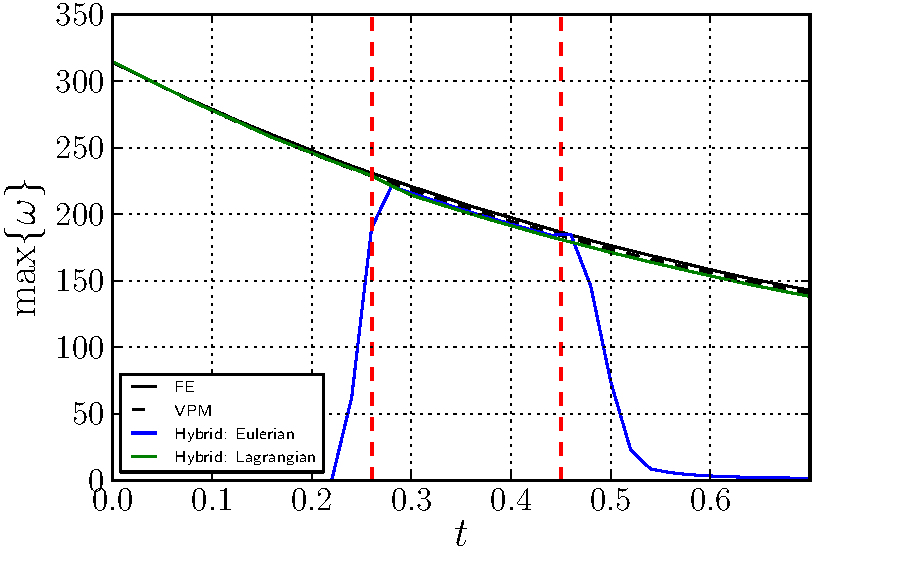
\includegraphics[width=\linewidth]{./figures/hybrid/cbConv/hybrid_dipoleConvection_hybridSubDomains_wMax.pdf}
             \caption{Discrep ???}
             \label{fig:hybrid_dipoleConvection_hybridSubDomains_wMax}
     \end{subfigure}     
     ~ %\qquad
     \begin{subfigure}[t]{0.48\textwidth}
             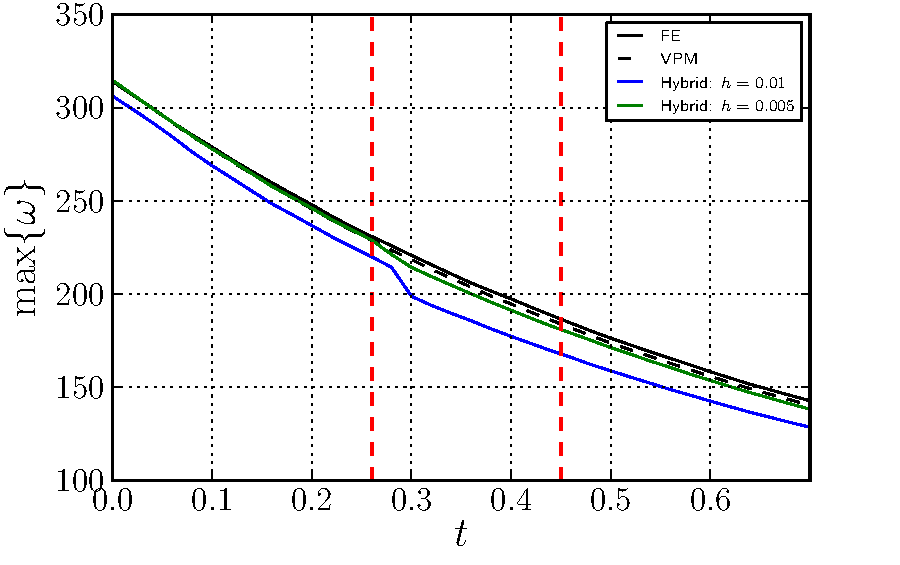
\includegraphics[width=\linewidth]{./figures/hybrid/cbConv/hybrid_dipoleConvection_comparison_parameter_wMax.pdf}
             \caption{Discrep ???}
             \label{fig:hybrid_dipoleConvection_comparison_parameter_wMax}
     \end{subfigure}        
     
     \caption{Desctipsd ???}
     \label{fig:hybrid_dipoleConvection_comparison_wMax}
	\end{figure}	
	
At $t=0.26$, the maximum vorticity in the Eulerian domain of the hybrid method starts to increase. This signifies the entering of the vortex core. Similarly, at $t=0.45$, the maximum vorticity starts to decrease, signifying the exiting of the vortex core. We see that there is a slight drop in the maximum vorticity w.r.t to the FE only, and the VPM only simulation, as the dipole enters the Eulerian domain. Similarly, as the dipole exits, there a slight peak in the solution of the Eulerian domain. A possible explanation to this phenomena might be error due to the artificial vorticity at the boundary. In section \ref{}, we observed that error in coupling introduces artificial vorticity at the boundary and the strength of this vorticity is proportional to the error in coupling. 
	
	\begin{figure}[!h]
     \centering
     \begin{subfigure}[t]{0.48\textwidth}
             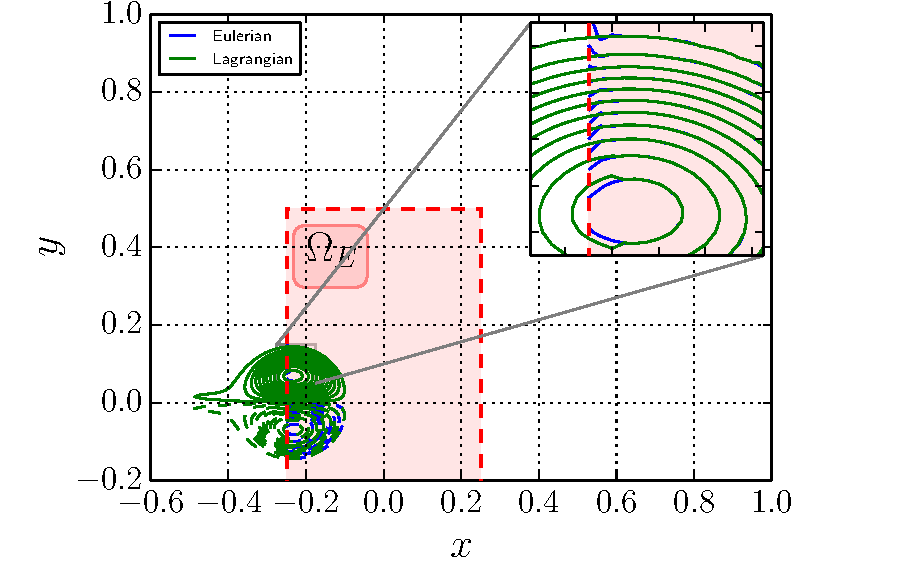
\includegraphics[width=\linewidth]{./figures/hybrid/cbConv/hybrid_doubleMonopoleConvection_entering2.pdf}
             \caption{Discrep ???}
             \label{fig:hybrid_doubleMonopoleConvection_entering2}
     \end{subfigure}     
     ~ %\qquad
     \begin{subfigure}[t]{0.48\textwidth}
             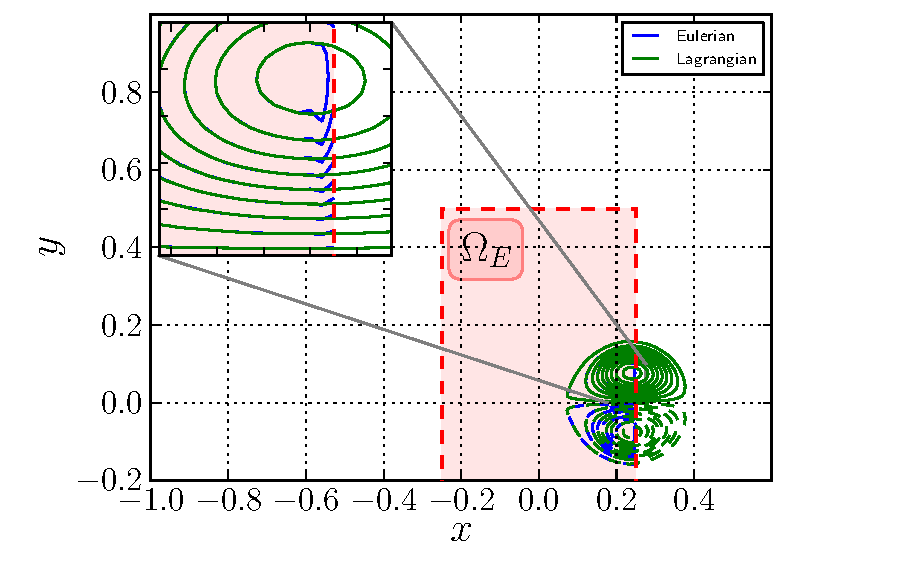
\includegraphics[width=\linewidth]{./figures/hybrid/cbConv/hybrid_doubleMonopoleConvection_exiting.pdf}
             \caption{Discrep ???}
             \label{fig:hybrid_doubleMonopoleConvection_exiting}
     \end{subfigure}        
     
     \caption{Desctipsd ???}
     \label{fig:hybrid_doubleMonopoleConvection_ent_exi}
	\end{figure}

Figure \ref{fig:hybrid_doubleMonopoleConvection_entering2} shows a vorticity contour plot of the Lagrangian method and the Eulerian method, at $t=0.28$ when the dipole has entered the Eulerian domain. We see that there is a mismatch in the vorticity at the boundary of the Eulerian domain. Similarly, there is a slight mismatch in the vorticity field when the dipole leaves the Eulerian domain, figure \ref{fig:hybrid_doubleMonopoleConvection_exiting}.

A simulation with lower Lagrangian resolution was ran to verify this theory. Figure \ref{fig:hybrid_dipoleConvection_comparison_parameter_wMax} compares the evolution of maximum vorticity $\omega_{max}$ for nominal blob spacing $h=0.01$ and $h=0.005$. The less resolved simulation shows a larger drop in maximum vorticity during the entry of the dipole. However, at $t=0.45$, the exiting of the dipole has no effect on the maximum vorticity. 

The evolution of the kinetic energy $E$ and the enstrophy $\Omega$ shows the same behavior, figure \ref{fig:hybrid_dipoleConvection_comparison_parameter_E} and  \ref{fig:hybrid_dipoleConvection_comparison_parameter_Omega}, respectively. It shows that during the entry there is larger change in the kinetic energy and the enstrophy of the flow. This means that the artificial vorticity causes increased diffusion of the flow. Therefore, with the reduced strength of the vortex core, the dipole should travel should have less energy and travel slower, which is observed in figure \ref{fig:hybrid_doubleMonopoleConvection_contourfPlots}. The effect is more sever for a lower resolved Lagrangian method, as seen for the simulation with $h=0.01$.

	\begin{figure}[!t]
     \centering
     \begin{subfigure}[t]{0.48\textwidth}
             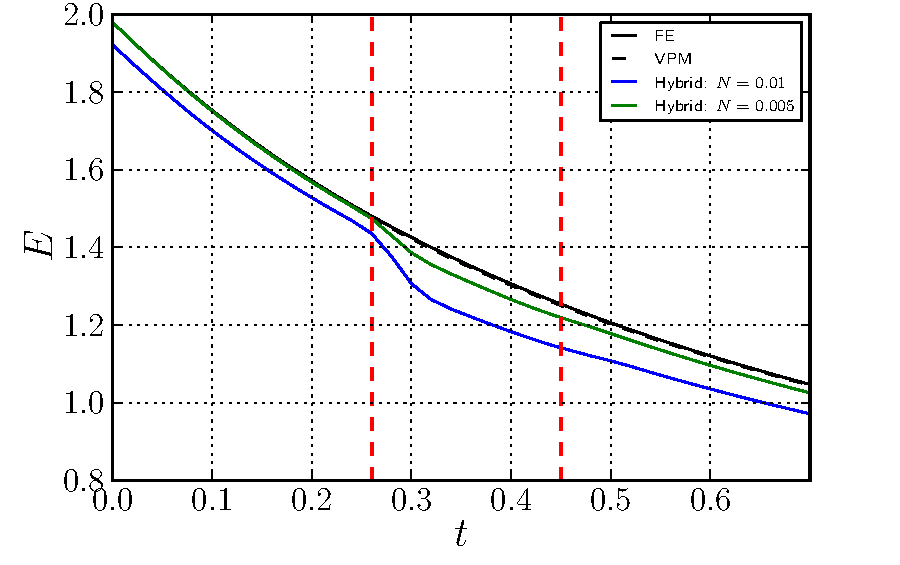
\includegraphics[width=\linewidth]{./figures/hybrid/cbConv/hybrid_dipoleConvection_comparison_parameter_E.pdf}
             \caption{Discrep ???}
             \label{fig:hybrid_dipoleConvection_comparison_parameter_E}
     \end{subfigure}     
     ~
     \begin{subfigure}[t]{0.48\textwidth}
             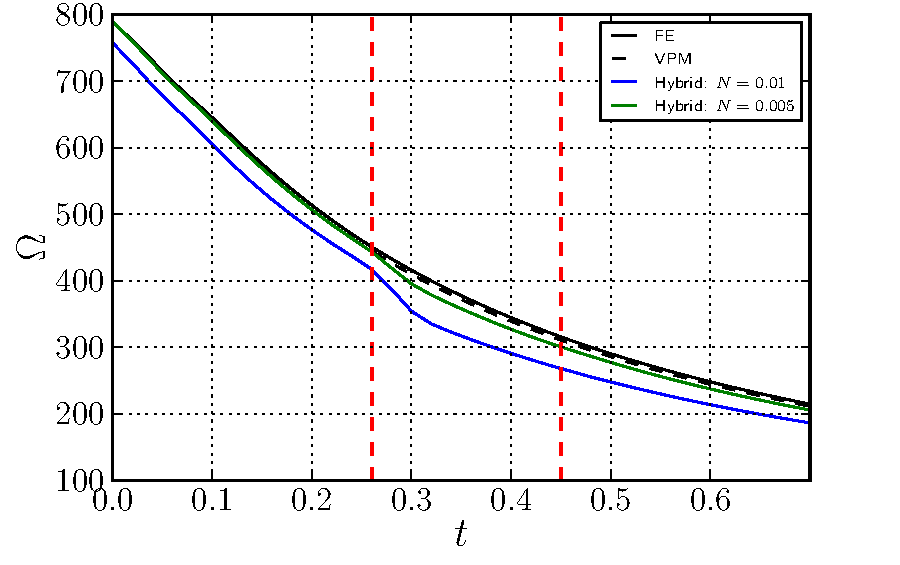
\includegraphics[width=\linewidth]{./figures/hybrid/cbConv/hybrid_dipoleConvection_comparison_parameter_Omega.pdf}
             \caption{Discrep ???}
             \label{fig:hybrid_dipoleConvection_comparison_parameter_Omega}
     \end{subfigure}        
     
     \caption{Desctipsd ???}
     \label{fig:hybrid_dipoleConvection_comparison_parameter}
	\end{figure}

\subsection{Conclusion}

In conclusion, we see that a high resolution discretization of the Lagrangian method inside the Eulerian domain $\Omega_L \cap \Omega_E$ is paramount for accurate transfer of information to and from the Eulerian method. For a lower resolved Lagrangian method in this region introduces artificial vorticity at the boundary of the Eulerian domain $\Sigma_d$, corrupting the solution of the coupling.

\section{Clercx-Bruneau Dipole Collision}

In this section, we study the Clercx-Bruneau dipole colliding with a solid wall. A Finite Element (FE) only investigate was performed in section . The purpose of the Clercx-Bruneau dipole collision investigate how the hybrid method deal with wall bounded problem. It was determined the FE only simulation able to accurately simulate the test cases, with the validation data provided by Clercx and Bruneau \cite{Clercx2006a}. Therefore, with help of the these data, we can verify the validate the wall-bounded problem.

\subsection{Problem Definition}

The description of the Clercx-Bruneau dipole collision problem was introduced in section \ref{subsec:eul_cbdc}. However now, the problem is simulated using the hybrid method. Figure ?? shows the step-up of the simulation, with Eulerian domain $\Omega_E$ resolving the near-wall region, and the Lagrangian domain resolving the complete fluid domain. The fluid domain is bounded by the no-slip wall $\Sigma_{wall}$ (shown in blue). The Eulerian domain $\Omega_E$ extends from the wall $\Sigma_{wall}$ to the boundary $\Sigma_{d}$, where Dirichlet velocity is prescribed. The parameters of the domain are tabulated in table \ref{tab:h_clercxBruneauParameters}.

	\begin{figure}[!h]
	\showthe\columnwidth
	\centering
	%\includegraphics[trim=0cm 2.5cm 0cm 2.5cm, clip, width=\linewidth]
	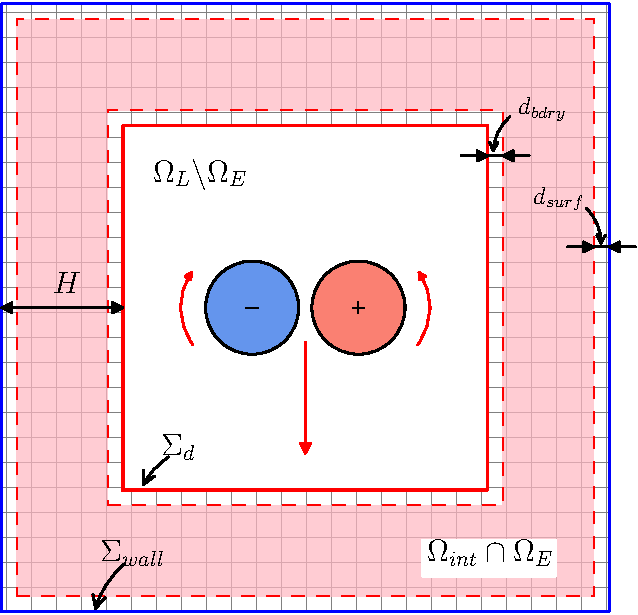
\includegraphics[width=0.5\linewidth]{./figures/hybrid/cbColl/hcbdc_dd-crop.pdf}
	\caption{[\textit{Not to Scale}] The domain decomposition for the Clercx-Bruneau dipole collision problem, with the positive pole at $p_{+}=(x_1,y_1) = (0.1,0)$ and negative pole at $p_{-}=(x_2,y_2)=(-0.1,0)$. The parameters of the simulation are tabulated in table \ref{tab:h_clercxBruneauParameters}.}
	\label{fig:hcbdc_dd}
	\end{figure}

As we are dealing with the wall-bounded problem, we require the vortex panel method to enforce the boundary condition in the Lagrangian method. In section \ref{sec:dotd} we described the decomposition of the Lagrangian domain $\Omega_L$ to the vortex blob domain $\Omega_b$ and the vortex panel domain $\Omega_p$. This decomposition was applied to this problem, as shown in figure \ref{fig:hcbdc_dd}.

	\ctable[
		caption = {Summary of the parameters for the Clercx-Bruneau dipole collision.},
		label   = {tab:h_clercxBruneauParameters},
		pos = !t,]{lcll}{}{\FL
		Parameters					& Value 				& Unit		& Description \ML
		$\Omega$               		& $\left[-1,1\right]^2$ &\si{m}		& Eulerian domain bounds \\
		$H$ & 0.2 & \si{m} & Eulerian domain width\\
		$Re$  			       		& $625$ 				&-			& Reynolds number \\ 
		$U$							& 1 & \si{m.s^{-1}} & Characteristic velocity\\
		$W$							& 1 & \si{m} & Characteristic Length\\
		$\nu$						& $\num{1.6e-3}$ 		&\si{kg.s^{-1}.m^{-1}}& Kinematic viscosity\\
		$ (x,y)_{1,2}$				& $(\pm0.1,0)$			& \si{m}    & Initial location of the dipole\\
		$\omega_e$					& 299.528385375226 & - & Characteristic vorticity of the monopole \cite{Renac2013}\\
		$\lambda$					& 1 & - & Overlap ratio\\
		$h$							& 0.003 & \si{m} & Nominal blob spacing\\
		$N_{panels}$ & 400 & - & Number of panels\\
		$h_{grid}$ 					& $0.005$ to $0.01$ & \si{m}	& FE cell diameter \\	
		$ N_{\mathrm{cells}}$ 		& $58272$ 	& -						& Number of mesh cells\\	
		$\Delta t_L$				& \num{2.5e-4} & \si{s} & Lagrangian time step size\\
		$\Delta t_E$				& \num{2.5e-5} & \si{s} & Eulerian time step size\\		
		$k_E$						& 10 & - & Eulerian sub-steps\\			
		$ N_{\mathrm{t-steps}}$ 	& 4000 & -			& Number of time integration steps\\
		$t$							& 0 to 1 & - & Simulation time\\
		$d_{bdry}$					& $2\cdot{h}$ & \si{m} & Interpolation boundary offset\\
		$d_{surf}$					& $3\cdot{h}$ & \si{m} & Interpolation offset at surface\LL}		

The parameters of the simulation follows are similar to the ones used in the FE only investigation, section \ref{subsec:eul_cbdc}, and are tabulated in table \ref{tab:h_clercxBruneauParameters}. The dipole is initialized in the center of the domain, in the Lagrangian only domain $\Omega_L\backslash\Omega_E$ at $(x,y)_{1,2}$. The dipole travels along the negative $y$-axis, entering the Eulerian domain $\Omega$ and finally colliding with the no-slip wall $\Sigma_{wall}$.

\subsection{Results and Discussion}

Figure \ref{fig:hybrid_doubleMonolope_contourfComparison} shows the state of the dipole at $t=[0,0.2,0.4,0.6,0.8,1]$. The figure compares the hybrid simulation (left half) with the FE only simulation (right half) from section \ref{subsec:eul_cbd}. Onces the dipole enters the Eulerian domain, $t=0.4$, we observe that there is a slight difference in the solution. The results loose the symmetry and there exists artifact vorticity at the Dirichlet boundary $\Sigma_d$. This emanating vorticity ($<\pm10$ with $\max\{\omega\}=320$) slight corrupts the solution of the collision. !!! APPENDIX !!!

Figure \ref{fig:hybrid_vorticity_contour_comparison} compares the vorticity contour at $t=1$ with the solution of Clercx and Bruneau. We see that he vorticity contours of hybrid has a slight difference with the solution of the FE only solution, figure \ref{fig:hybrid_dipole_contourLine_t1p0}. The shape of the contour lines near the wall is slightly different, and the location of the core is also shifted slightly.

	\begin{figure}[!p]
	\showthe\columnwidth
	\centering
	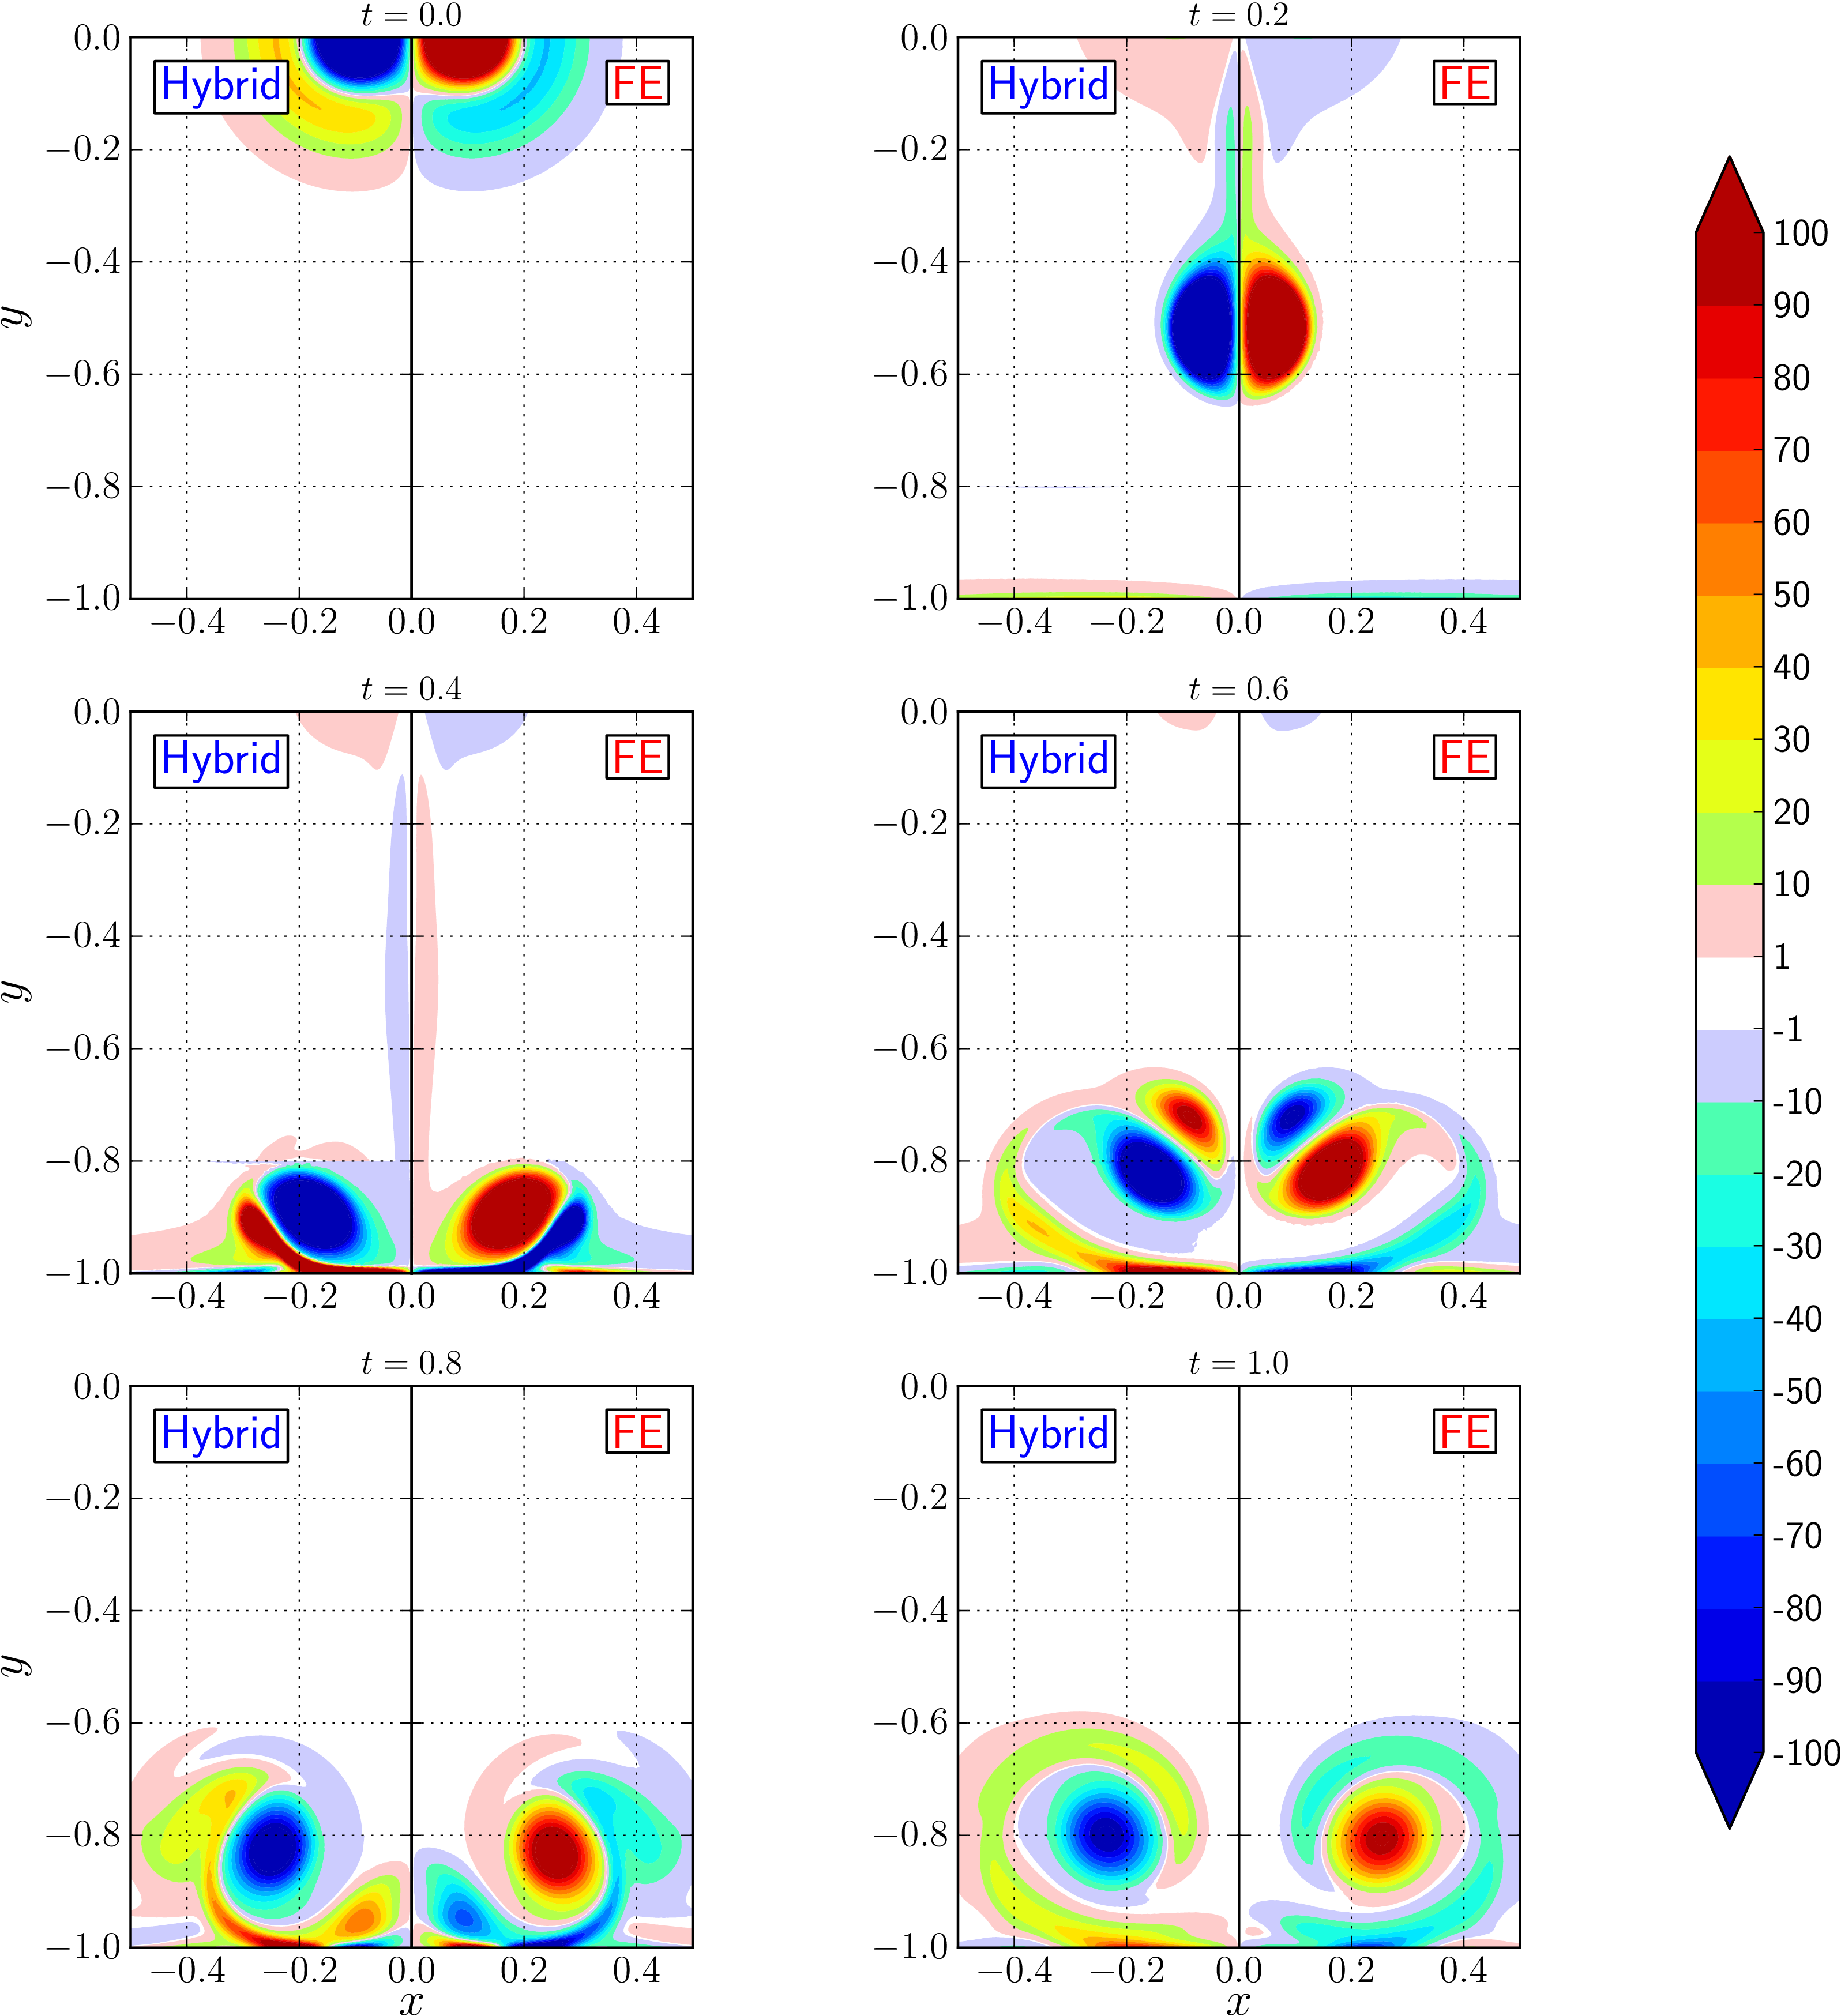
\includegraphics[width=\linewidth]{./figures/hybrid/cbColl/hybrid_doubleMonolope_contourfComparisonNew_compressed-crop.png}
	\caption{Plot of the dipole at $t = [0, 0.2, 0.4, 0.6, 0.8, 1]$, comparing the hybrid simulation (left half) and FE only simulation (right half).}
	\label{fig:hybrid_doubleMonolope_contourfComparison}
	\end{figure}

	\begin{figure}[!p]
     \centering
     \begin{subfigure}[t]{0.4\textwidth}
             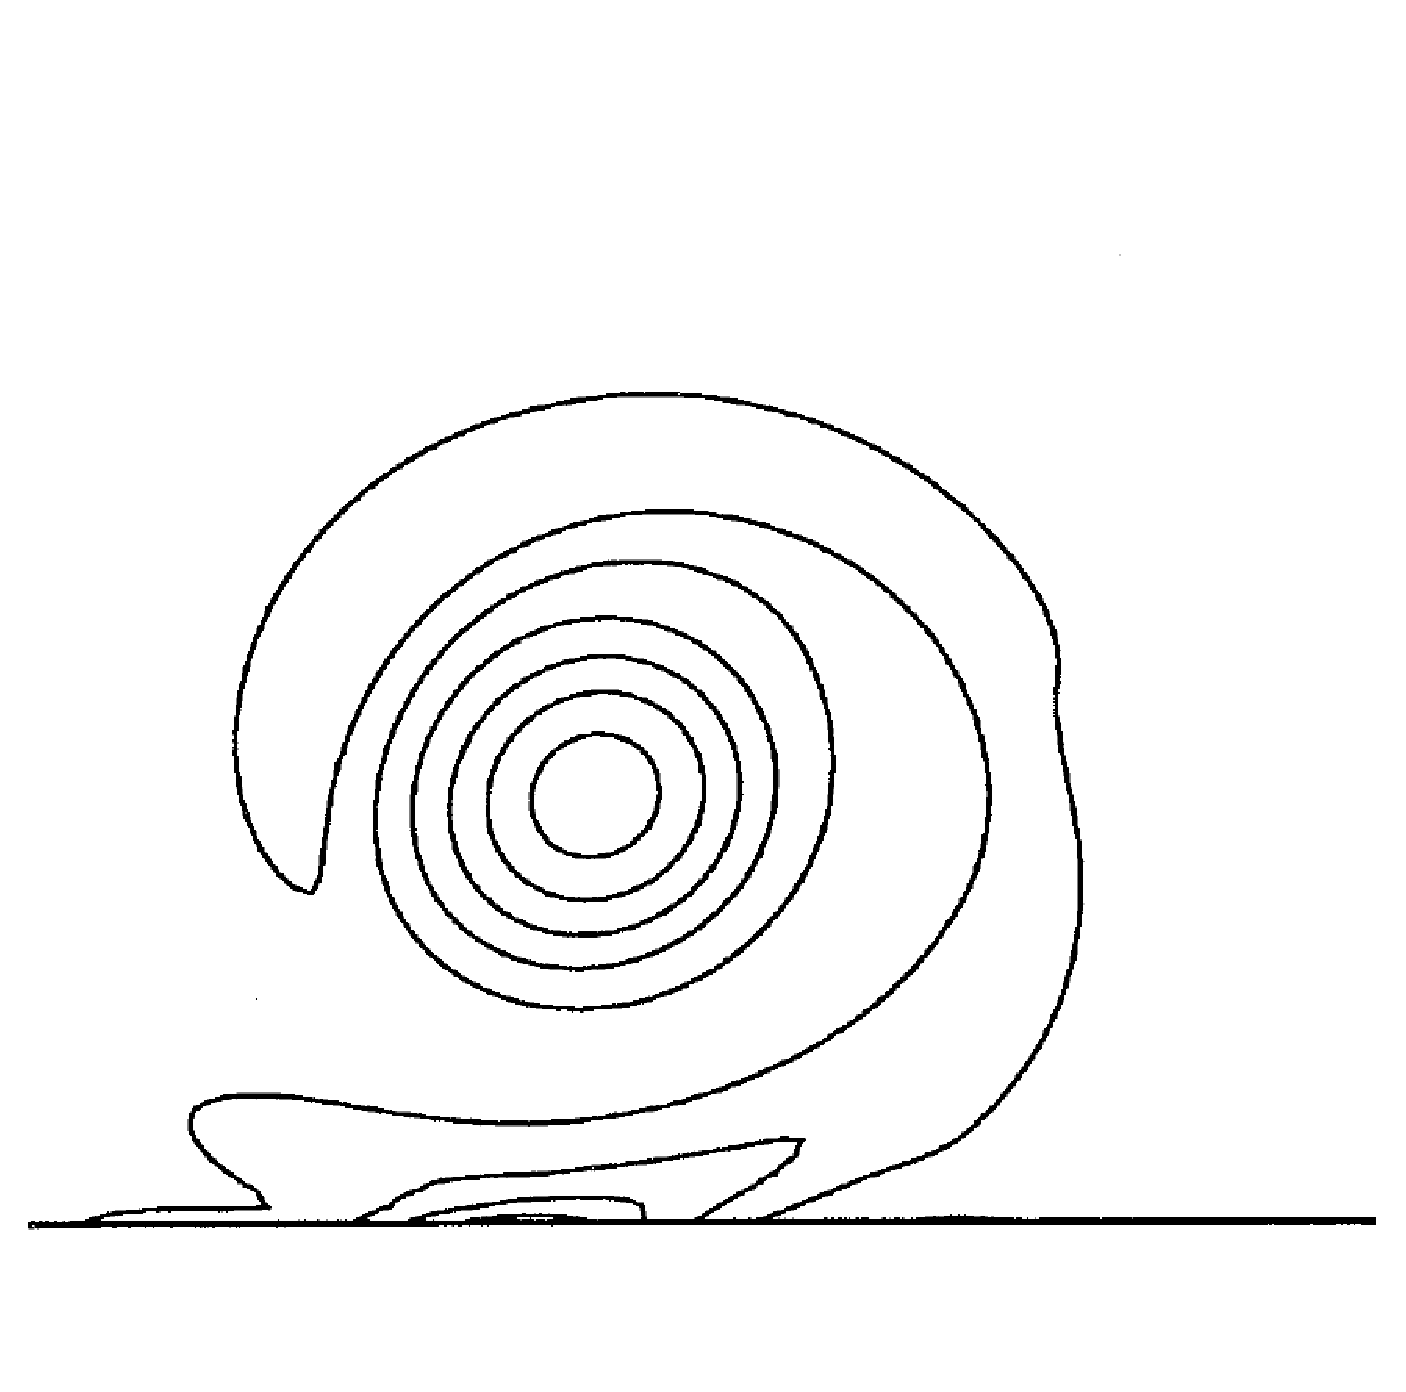
\includegraphics[width=\textwidth]{figures/eulerian/VorticityContourPlot-rotated270.pdf}
             \caption{Literature}
             \label{fig:hybrid_VorticityContourPlot}
     \end{subfigure}%
     ~ %add desired spacing between images, e. g. ~, \quad, \qquad etc.
       %(or a blank line to force the subfigure onto a new line)
     \begin{subfigure}[t]{0.5\textwidth}
             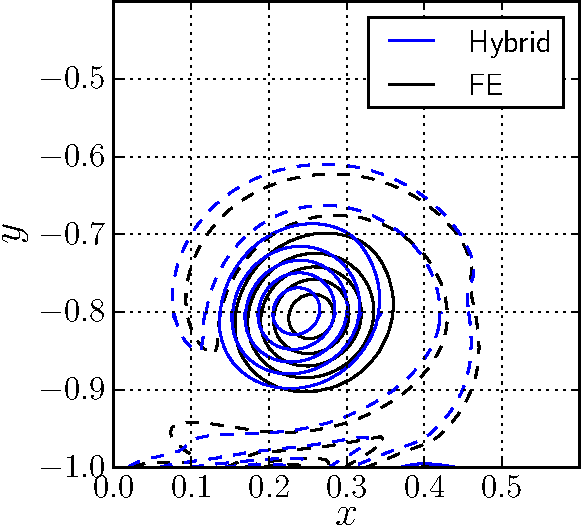
\includegraphics[width=\textwidth]{./figures/hybrid/cbColl/hybrid_doubleMonolope_contourComparison_t1-crop.pdf}
             \caption{Present study}
             \label{fig:hybrid_dipole_contourLine_t1p0}
     \end{subfigure}
     \caption{Comparison of the vorticity contours at $t=1$. The figure compares the plot obtained by \textbf{(a)} literature, Clercx and Bruneau \cite{Clercx2006a}, and \textbf{(b)} the present study, the hybrid and FE only simulation.}
     \label{fig:hybrid_vorticity_contour_comparison}
	\end{figure}	

	\begin{figure}[!p]
     \centering
     \begin{subfigure}[t]{0.49\textwidth}
             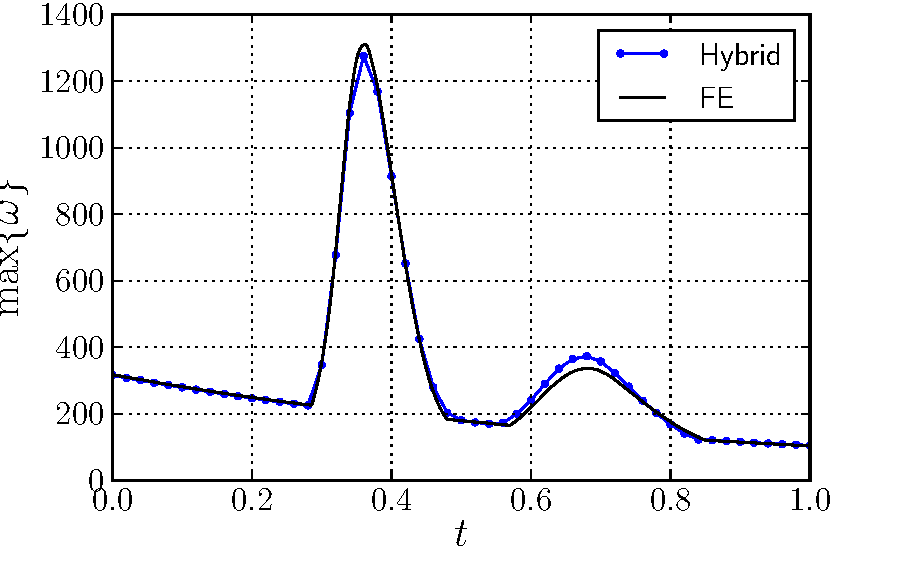
\includegraphics[width=\textwidth]{./figures/hybrid/cbColl/hybrid_doubleMonopole_parameter_wMax.pdf}
             \caption{Maximum vorticity $\max\{\omega\}$}
             \label{fig:hybrid_dipole_maxVorticity_comparison}
     \end{subfigure}%
     ~ %add desired spacing between images, e. g. ~, \quad, \qquad etc.
       %(or a blank line to force the subfigure onto a new line)
     \begin{subfigure}[t]{0.49\textwidth}
             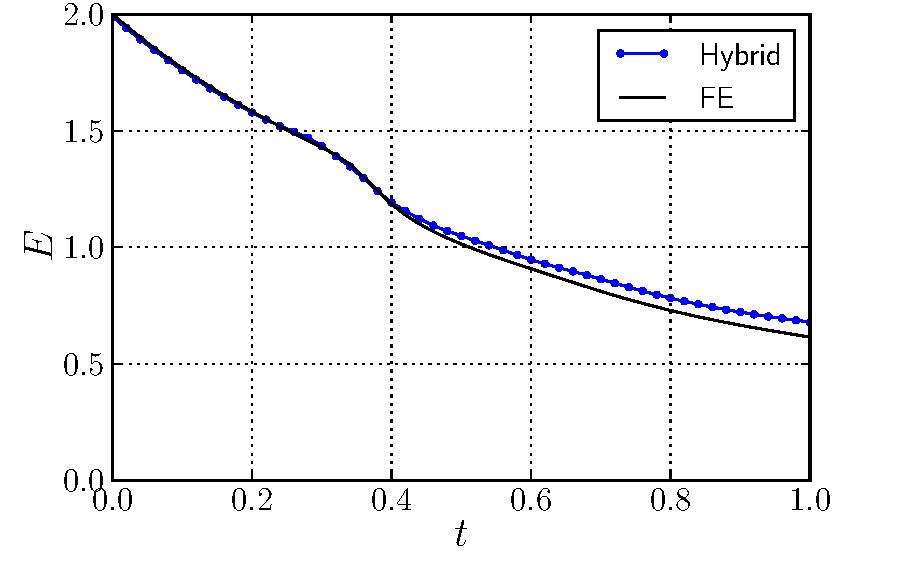
\includegraphics[width=\textwidth]{./figures/hybrid/cbColl/hybrid_doubleMonopole_parameter_E.pdf}
             \caption{Kinetic Energy $E(t)$}
             \label{fig:hybrid_dipole_KineticEnergy_comparison}
     \end{subfigure}
     
     \begin{subfigure}[b]{0.49\textwidth}
             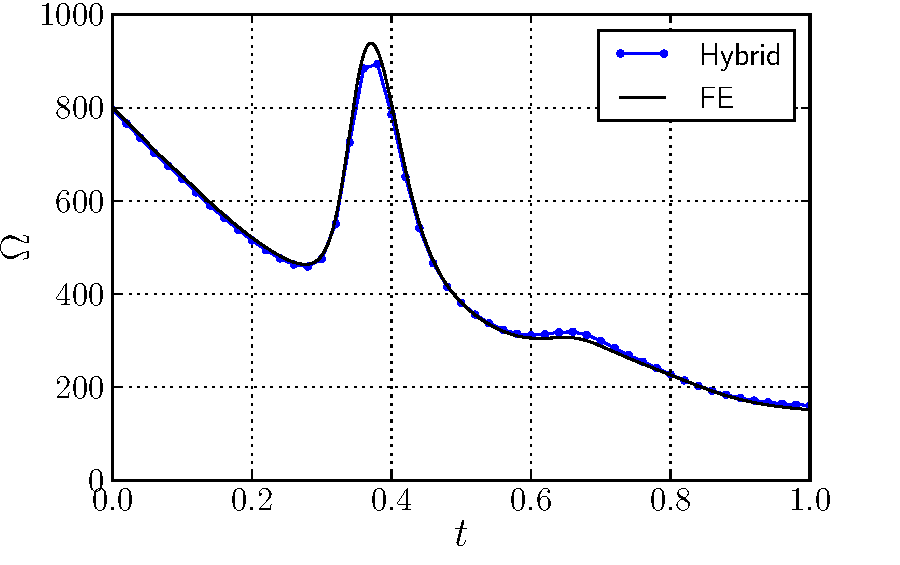
\includegraphics[width=\textwidth]{./figures/hybrid/cbColl/hybrid_doubleMonopole_parameter_Omega.pdf}
             \caption{Enstrophy $\Omega(t)$}
             \label{fig:hybrid_dipole_Enstrophy_comparison}
	 \end{subfigure}
     ~
	 \begin{subfigure}[b]{0.48\textwidth}
	 		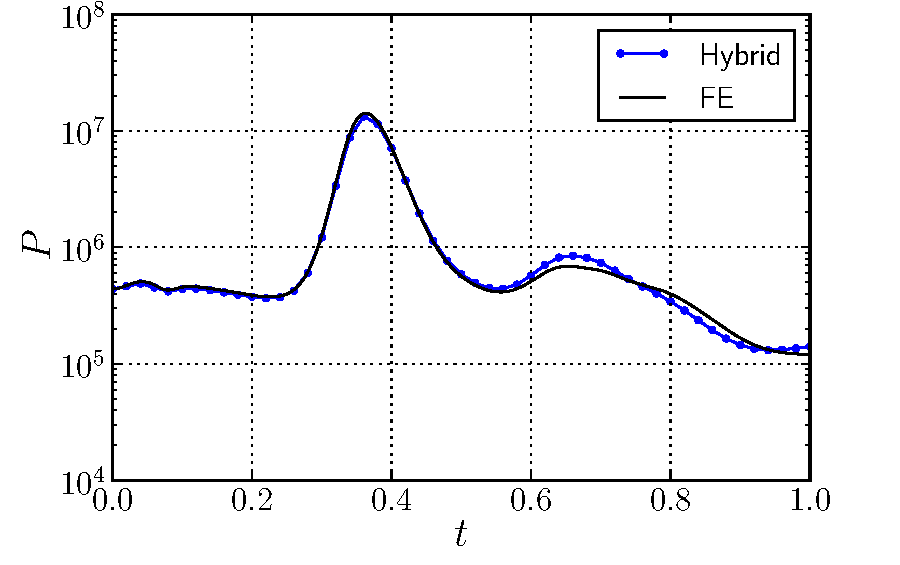
\includegraphics[width=\textwidth]{./figures/hybrid/cbColl/hybrid_doubleMonopole_parameter_P.pdf}
             \caption{Palinstrophy $P(t)$}
			\label{fig:hybrid_dipole_Palinstrophy_comparison}
	 \end{subfigure}     
     
     \caption{Comparison of the fluid parameters. Figure \textbf{(a)}, \textbf{(b)}, \textbf{(c)}, \textbf{(d)}compares the evolution of the fluid properties from $t=0$ to $t=1$.} %Figure \textbf{(d)} compares the vorticity generated at the bottom-left wall ($y=-1$, $-0.6\leqslant x \leqslant 0$) at $t=0.4$ [{\color{plotBlue}{---}}, solid blue], $t=0.6$ [{\color{plotRed}{---}}, solid red] and $t=1$ [{\color{plotGreen}{---}}, solid green].}
     \label{fig:hybrid_dipole_comparison}
	\end{figure}

To investigate further on the cause of this difference, we studied the change in maximum vorticity $\omega_{max}$, kinetic energy $E$ and enstrophy $\Omega$, and palinstrophy $P$, figure \ref{fig:hybrid_dipole_Palinstrophy_comparison}. The variation in maximum vorticity, figure \ref{fig:hybrid_dipole_maxVorticity_comparison}, shows that first peak in hybrid is slightly lower than the FE only simulation, $t\approx 0.35$. However, the second peak in vorticity, at $t\approx0.65$ is higher than the standard simulation. Between $t=0.4$ and $t=0.6$, the dipole exits and renters the Eulerian domain, as seen in figure \ref{fig:hybrid_doubleMonolope_contourfComparison}. This has a detrimental effect on overall vorticity field solution. 

Figure \ref{fig:hybrid_dipole_KineticEnergy_comparison} shows that, as the dipole leaves the Eulerian domain $\Omega_E$ from $t=0.4$, the kinetic energy $E$ reduces slower, and is higher than the FE only simulation for $t\leq0.4$. Therefore, the core that is leaving and re-entering the Eulerian domain $\Omega_E$ has a higher kinetic energy $E$. This could be cause of deviation seen at $t=1$, figure \ref{fig:hybrid_vorticity_contour_comparison}.

Figure \ref{fig:hybrid_dipole_Enstrophy_comparison} shows the enstrophy $\Omega$ matches reasonable well with the FE only simulation and we see that there is a slight difference at the peaks. Similarly, figure \ref{fig:hybrid_dipole_Palinstrophy_comparison}, shows the variation in palinstrophy $P$. The solution stars to deviate from $t\approx0.5$, after the vortex core re-enters the domain.

Figure \ref{fig:hybrid_doubleMonopole_vorticityAtBoundary} shows the vorticity at the boundary, along $y=-1$. We observe that for $t=0.4$ the solution matches, at $t=0.6$ the peak in vorticity is larger for the hybrid simulation, and for $t=1$, the peak has a larger span. The increased kinetic energy $E$ of the vortex could provide a possible explanation for this. With a higher kinetic energy, the wall has to generate more vorticity to enforce the no-through flow.

	\begin{figure}[!t]
	\showthe\columnwidth
	\centering
	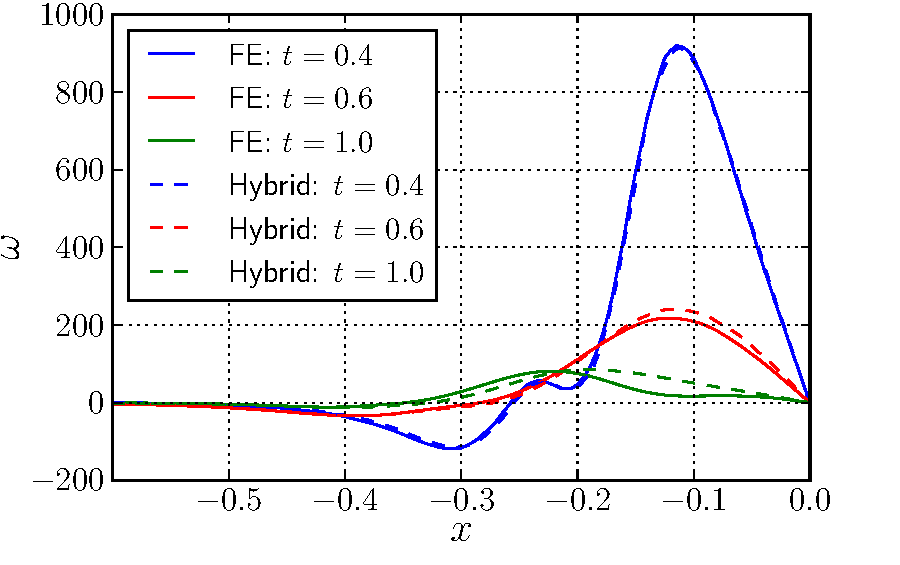
\includegraphics[width=0.5\linewidth]{./figures/hybrid/cbColl/hybrid_doubleMonopole_vorticityAtBoundary.pdf}
	\caption{Compares the vorticity generated at the bottom-left wall ($y=-1$, $-0.6\leqslant x \leqslant 0$) at $t=0.4$ [{\color{plotBlue}{---}}, solid blue], $t=0.6$ [{\color{plotRed}{---}}, solid red] and $t=1$ [{\color{plotGreen}{---}}, solid green].}
	\label{fig:hybrid_doubleMonopole_vorticityAtBoundary}
	\end{figure}

To determine, the effects of parameters, we investigated that for higher resolved Lagrangian field with smaller nominal blob spacing $h$, larger number of panels $N_{panels}$ and smaller Lagrangian time step size $\Delta t_L$. However, the results of these simulation provided only a slight improvement w.r.t the present investigation. Therefore, we see that the primary source of the error in not the resolution of the Lagrangian solution, but entering and re-entering of the vorticity into the Eulerian domain.


\subsection{Conclusion}

In conclusion, we determined that the exists a slight difference in the geometry of the vorticity contours and the location of the dipole at the end of the simulation. The deviation of the dipole stars as the dipole enters the Eulerian domain. The entering and the re-entering process of the dipole introduces artificial vorticity from the Dirichlet boundary $\Sigma_d$, increasing the overall kinetic energy $E$ of the problem. This intern has an influence on the position of the dipole at $t=1$. Increasing the resolution of the Lagrangian solution only minimally increases the accuracy of the results meaning that the source of the coupling of the solution itself.  


\section{Impulsively Started Cylinder at $Re=550$}

In this section, we will study the flow around an impulsively started cylinder at $Re=550$. The purpose of the this test case is ensure we are able to correctly predict the forces acting on the body. In section \ref{subsec:eul_isc}, a FE only simulation was ran, and we where able to determine the performance the FE simulation w.r.t to the literature data provided by Koumoutsakos and Leonard \cite{Koumoutsakos1995a}, and the data provide by  RosenFeld et al. \cite{MosheRosenFeldDochanKwak1991}. These investigations will be used as the benchmark for the upcoming study.

\subsection{Problem Definition}

The description of the impulsively started test case was given in section \ref{subsec:eul_isc}. For the hybrid simulation, we performed similar investigated and the compared with the validation data. The parameters of the simulation are tabulated in table \ref{tab:h_ISCParameters}. 

	\ctable[
		caption = {Summary of the parameters of the hybrid simulation for the Impulsively started cylinder test case for $Re=550$.},
		label   = {tab:h_ISCParameters},
		pos = !p,]{lcll}{}{\FL
		Parameters					& Value 				& Unit		& Description \ML
		$Re$  			       		& $550$ 				&-			& Reynolds number \\ 
		$\mathbf{u}_{\infty}$		& $[1,0]$ 				&\si{m.s^{-1}}& Free-stream velocity\\		
		$R$			         		& $1$ 					&\si{m}		& Radius of cylinder\\		
 		$R_{ext}$ & 1.5 & \si{m} & Radius of Eulerian domain $\Omega_E$ \\
		$\nu$						& $\num{3.6e-3}$ 		&\si{kg.s^{-1}.m^{-1}}& Kinematic viscosity\\
		$\lambda$					& 1 & - & Overlap ratio\\
		$h$							& 0.008 & \si{m} & Nominal blob spacing\\		
		$h_{grid}$ 					& $0.008$ to $0.04$ & \si{m}	& FE cell diameter \\
		$ N_{\mathrm{cells}}$ 		& $32138$ 	& -						& Number of mesh cells\\						
		$N_{panels}$ & 100 & - & Number of panels\\
		$\Delta t_L$				& 0.005 & \si{s} & Lagrangian time step size\\
		$\Delta t_E$				& 0.001  & \si{s} & Eulerian time step size\\		
		$k_E$						& 5 & - & Eulerian sub-steps\\			
		$ N_{\mathrm{t-steps}}$ 	& 40000 & -			& Number of time integration steps\\
		$t$							& 0 to 40 & - & Simulation time\\
		$d_{bdry}$					& $0.1\cdot{R}$ & \si{m} & Interpolation offset from boundary $\Sigma_d$\\
		$d_{surf}$					& $3\cdot{h}$ & \si{m} & Interpolation offset from boundary $\Sigma_{wall}$\LL}

Figure \ref{fig:hisc_dd} shows the domain decomposition of the hybrid simulation. The Eulerian domain $\Omega_E$ is bounded by boundary $\partial\Omega_E$, where $\partial\Omega_E=\Sigma_d\cup\Sigma_{wall}$, where $\Sigma_d$ is the external Dirichlet boundary and $\Sigma_{wall}$ is the no-slip wall. The Lagrangian domain $\Omega_L$ resolves the full fluid domain. The interpolation region $\Omega_{int}$, where we correct the particle strengths is within the Eulerian domain $\Omega_E$, such that $\Omega_{int}\subset\Omega_E$. The interpolation region $\Omega_{int}$ is bounded by $\partial\Omega_{int}$ where $\partial\Omega_{int}=\Sigma_p\cup\Sigma_{int;ext}$. The vortex panel boundary $\Sigma_p$ has an offset $d_{surf}=3\cdot{h}$ from the wall $\Sigma_{wall}$. The offset is chosen according to stock, see section \ref{}. The exterior boundary $\Sigma_{int;ext}$ of the interpolation region $\Omega_{int}$ is defined with a larger offset $d_{bdry} = 0.1\cdot{R}$. We observed in the previous sections that the main error of the hybrid scheme is the artificial vorticity generated at the $\Sigma_d$ and to reduce this error, we chose the larger offset.

	\begin{figure}[!h]
	\showthe\columnwidth
	\centering
	%\includegraphics[trim=0cm 2.5cm 0cm 2.5cm, clip, width=\linewidth]
	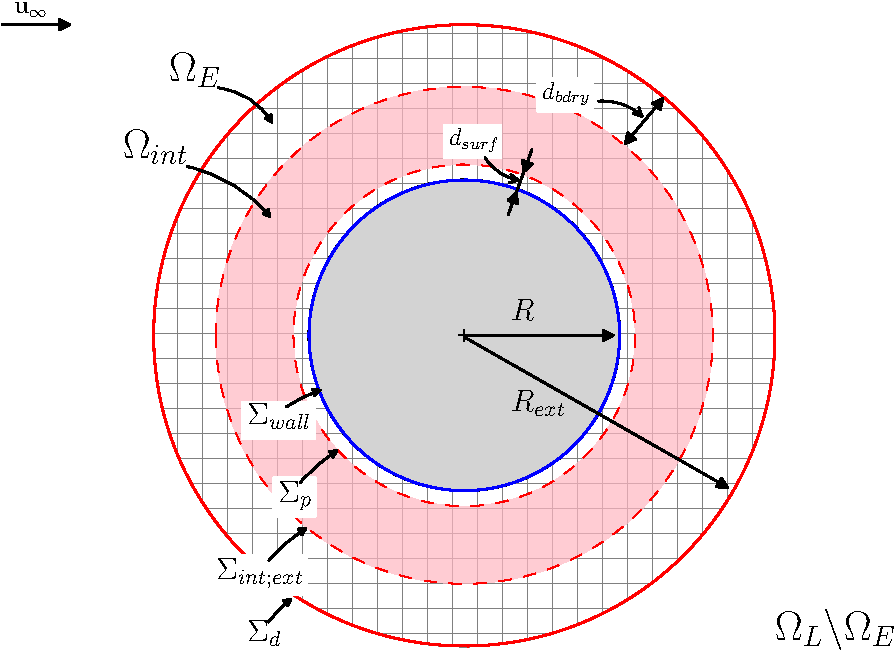
\includegraphics[width=0.6\linewidth]{./figures/hybrid/isc/hisc_dd-crop.pdf}
	\caption{[\textit{Not to Scale}] The domain decomposition for the Impulsively started cylinder. The parameters of the domain are tabulated in table \ref{tab:h_ISCParameters}.}
	\label{fig:hisc_dd}
	\end{figure}

The initial boundary conditions of the Eulerian Dirichlet boundary $\Sigma_d$, is the velocity field induced by the vortex panels. At time progress, the vorticity is generated from the Eulerian boundary $\Sigma_{wall}$, transferring to the vortex blobs inside the interpolation region $\Omega_{int}$. 

Two investigation where performed with the impulsively started problem. The first study focused on the impact of parameters on the lift and drag acting on the cylinder. The parameters of interest during this parameter sensitivity analysis were the number of vortex panels $N_{panels}$, nominal blob spacing $h$, time step size of the Lagrangian method $\Delta t_L$.

The second focus of the investigation was the long run performance of the forces acting of the cylinder. Artificial perturbation was induced as described in section \ref{subsec:eul_isc} to initiate vortex shedding at the initial stages of the simulation.

\subsection{Results and Discussion}

	\begin{figure}[!p]
     \centering
     \begin{subfigure}[t]{0.49\textwidth}
             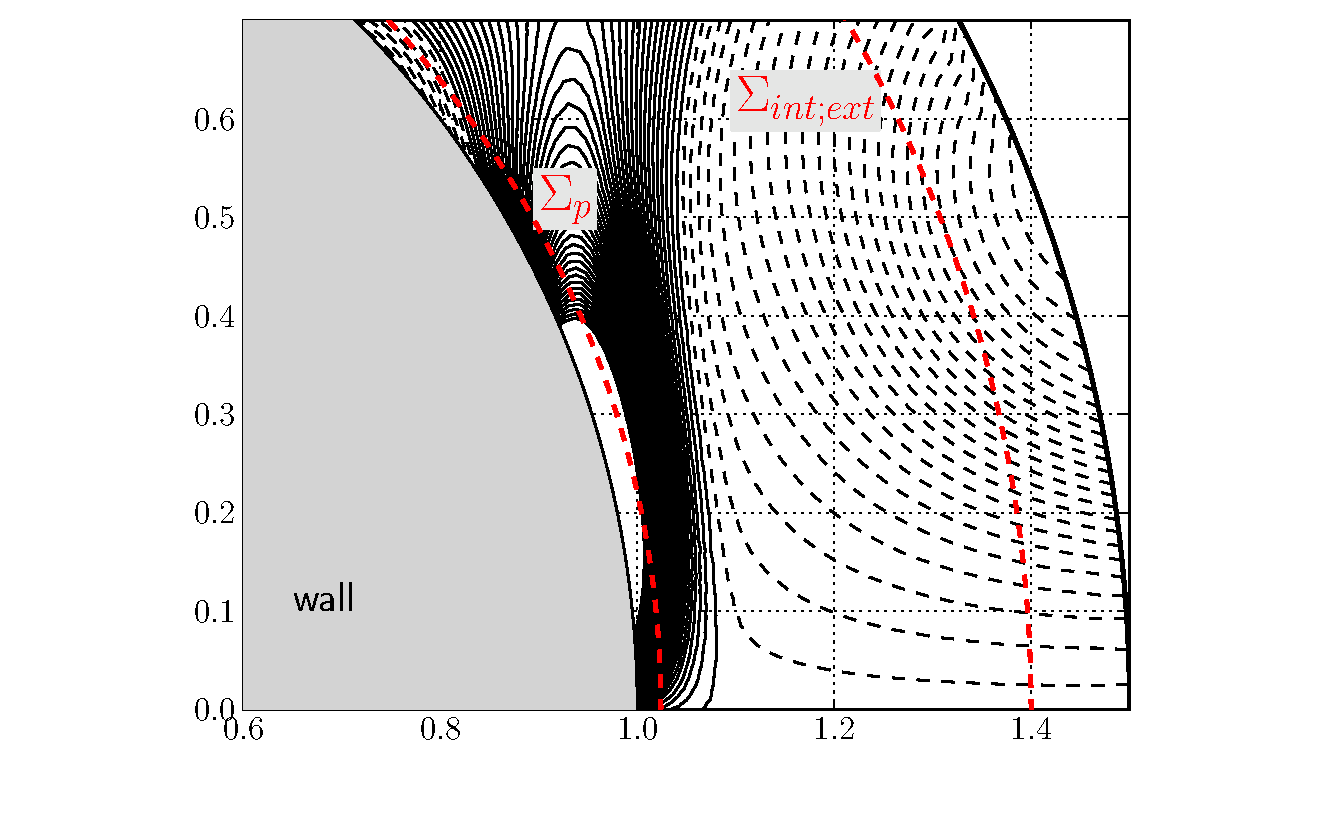
\includegraphics[width=\textwidth]{./figures/hybrid/isc/hisc_EulerianDomain_wall.pdf}
             \caption{Wall region: Eulerian method}
             \label{fig:hisc_EulerianDomain_wall}
     \end{subfigure}%
     ~ %add desired spacing between images, e. g. ~, \quad, \qquad etc.
       %(or a blank line to force the subfigure onto a new line)
     \begin{subfigure}[t]{0.49\textwidth}
             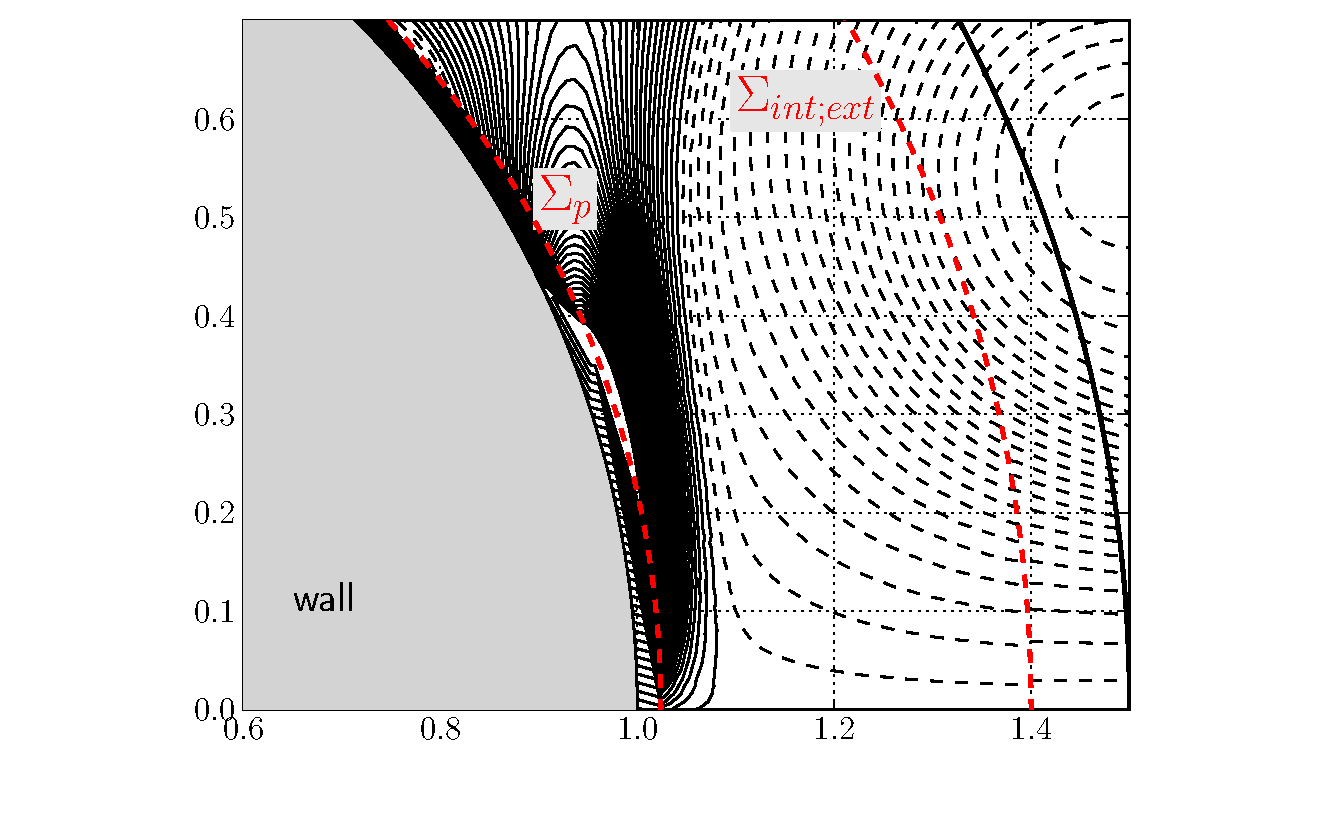
\includegraphics[width=\textwidth]{./figures/hybrid/isc/hisc_LagrangianDomain_wall.pdf}
             \caption{Wall region: Lagrangian method}
             \label{fig:hisc_LagrangianDomain_wall}
     \end{subfigure}
     
     \begin{subfigure}[t]{0.49\textwidth}
             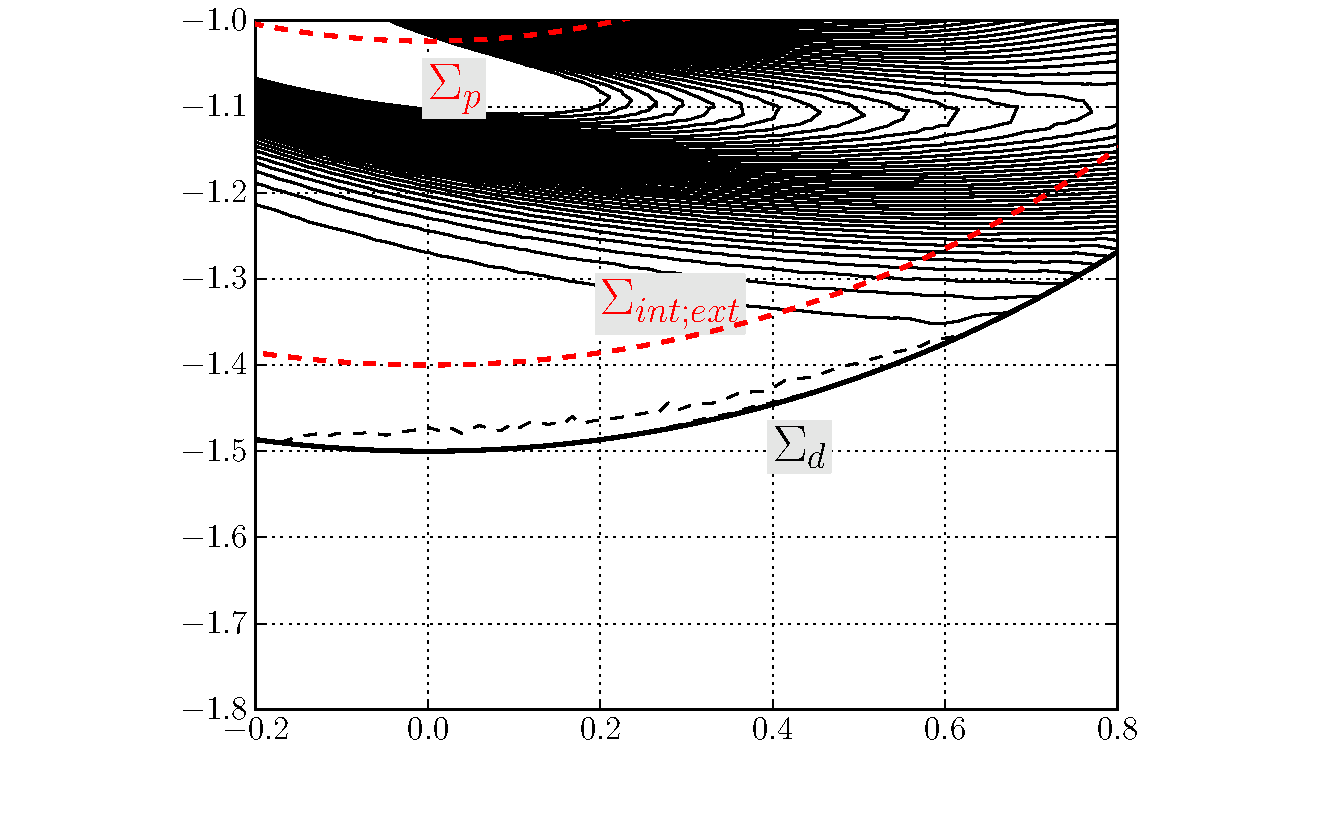
\includegraphics[width=\textwidth]{./figures/hybrid/isc/hisc_EulerianDomain_bdry.pdf}
             \caption{Boundary region: Eulerian method}
             \label{fig:hisc_EulerianDomain_bdry}
     \end{subfigure}%
     ~ %add desired spacing between images, e. g. ~, \quad, \qquad etc.
       %(or a blank line to force the subfigure onto a new line)
     \begin{subfigure}[t]{0.49\textwidth}
             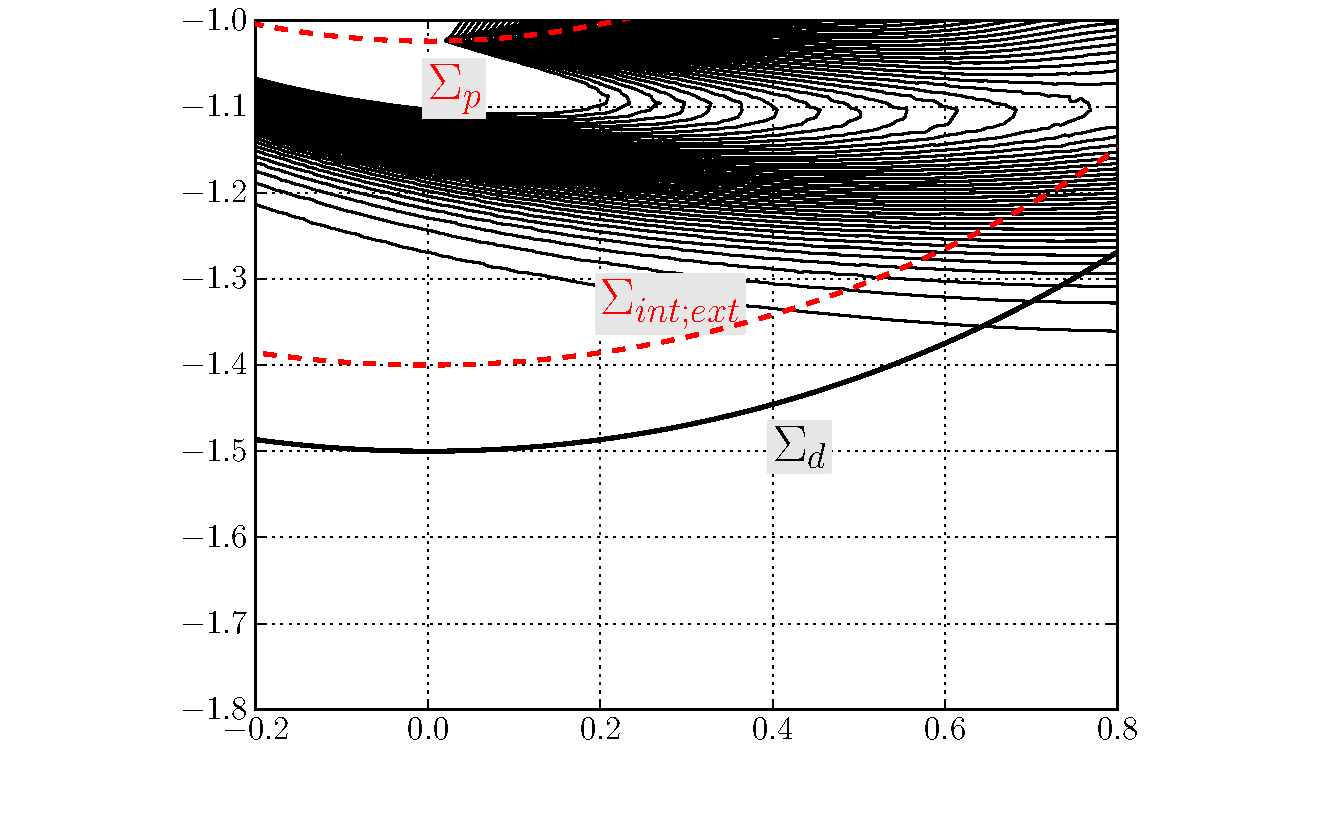
\includegraphics[width=\textwidth]{./figures/hybrid/isc/hisc_LagrangianDomain_bdry.pdf}
             \caption{Boundary region: Lagrangian method}
             \label{fig:hisc_LagrangianDomain_bdry}
     \end{subfigure}     
     \caption{Eulerian method and Lagrangian method resolutions}
     \label{fig:hisc_EulerianVsLagrangian}
	\end{figure}

Figure \ref{fig:hybrid_cylinder_contourComparison_tStarting} shows the vorticity contour at the initial stages of the simulation, $t = [1,3,5,7]$. The plot compares the hybrid simulation (top half) with the FE only simulation (bottom half). The hybrid half of the plot also depicts the Eulerian domain $\Omega_E$, and is bounded to the cylinder, resolving the near-wall region of the problem.

	\begin{figure}[!h]
	\showthe\columnwidth
	\centering
	%\includegraphics[trim=0cm 2.5cm 0cm 2.5cm, clip, width=\linewidth]
	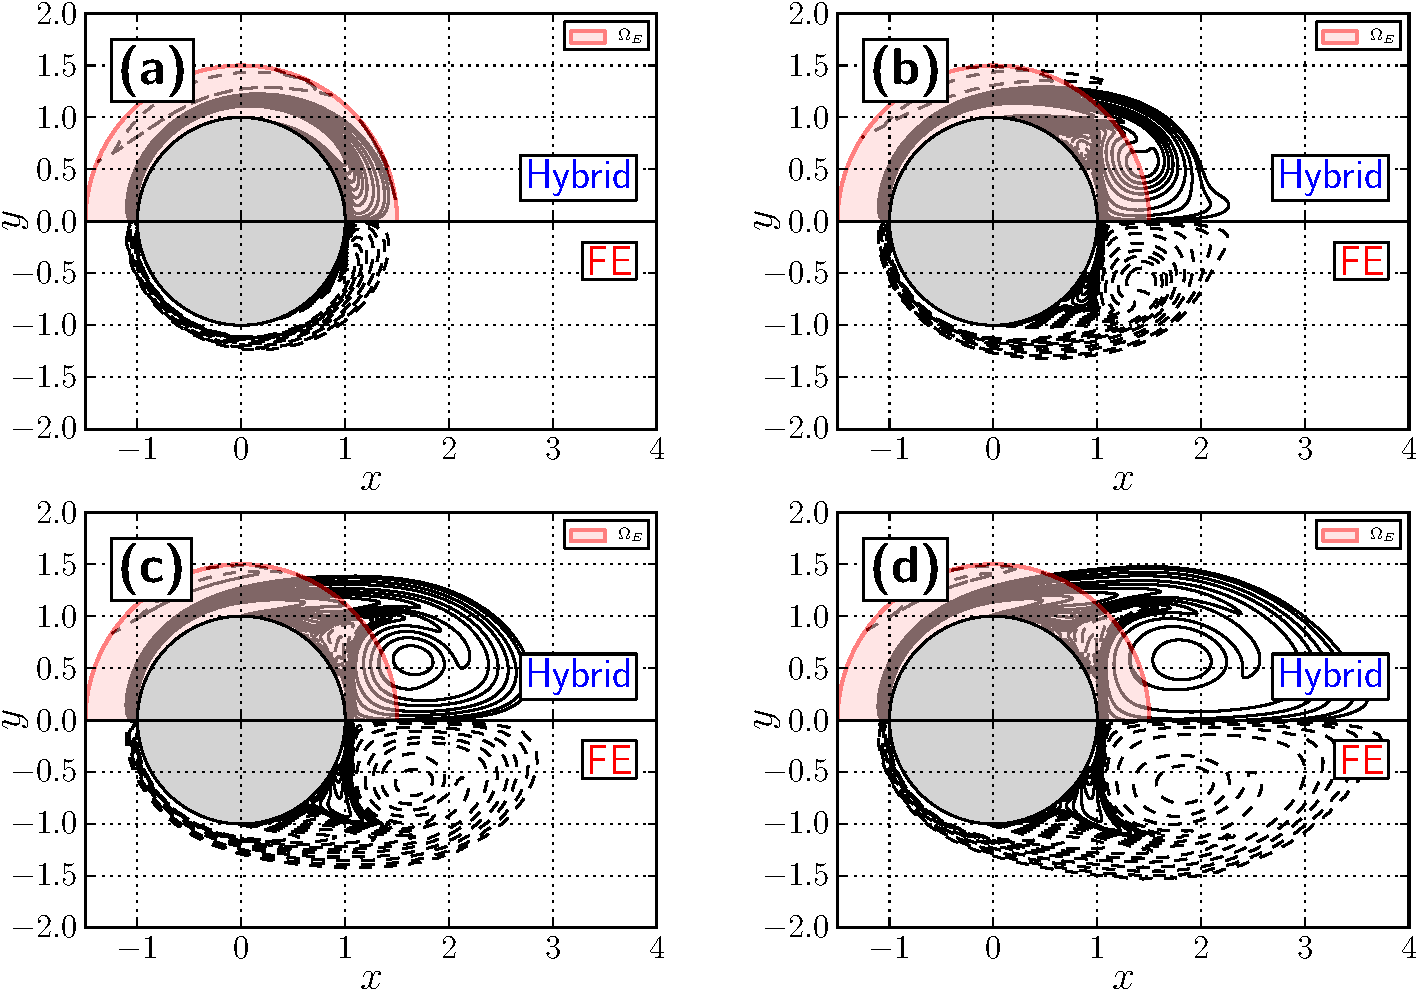
\includegraphics[width=\linewidth]{./figures/hybrid/isc/hybrid_cylinder_contourComparison_tStarting-crop.pdf}
	\caption{Comparison of the vorticity contours for \textbf{(a)} $t=1$, \textbf{(b)} $t=3$, \textbf{(c)} $t=5$ and \textbf{(d)} $t=7$ with contour levels [$-7,...,-3,-2,-1,0.5,-0.2,-0.1,0.1,0.2,0.5,1,2,3,...,7$]. The figures compares the hybrid simulation (top half) with FE only simulation (bottom half).}
	\label{fig:hybrid_cylinder_contourComparison_tStarting}
	\end{figure}

We observe that the vorticity contours of the hybrid simulation matches with the FE only simulation. The figure is nearly symmetric expect the artificial vorticity emanating from the Dirichlet boundary $\Sigma_d$, convecting with the free-stream. This magnitude of this artificial vorticity is within $|\omega|\leqslant0.2$ where the maximum vorticity in the domain is $\max\{\Omega\}=32$. Therefore, the relative vorticity generated from the boundary with less than $1\%$ of the maximum vorticity in the fluid.

	\begin{figure}[!p]
	\showthe\columnwidth
	\centering
	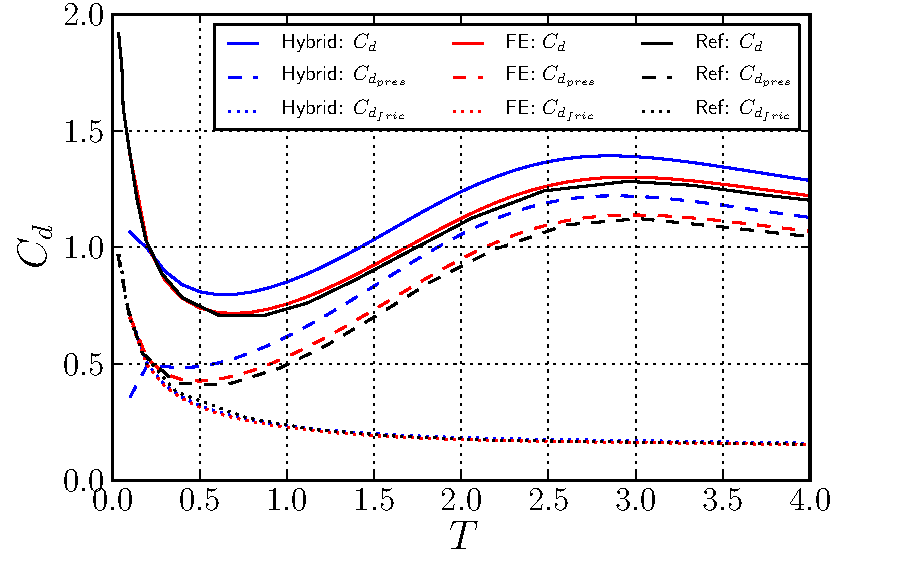
\includegraphics[width=0.6\linewidth]{./figures/hybrid/isc/hybrid_ISC_drag.pdf}
	\caption{ Evolution of the drag coefficient during the initial stages $t=0$ to $t=4$ with total drag coefficient $C_d$ (solid), pressure drag coefficient $C_{d_{pres}}$ (dashed) and friction drag coefficient $C_{d_{fric}}$ (dotted). The figure compares results of hybrid simulation ({\color{plotBlue}{\textbf{blue}}}), FE only simulation ({\color{plotRed}{\textbf{red}}}) and reference data (\textbf{black}) of Koumoutsakos and Leonard \cite{Koumoutsakos1995a}}
	\label{fig:hybrid_ISC_drag}
	\end{figure}

The investigate the effect of this error, we determined the error in the evolution of the drag during the initial stages of the simulation. Figure \ref{fig:hybrid_ISC_drag} shows the evolution of the drag coefficient $C_d$, friction drag $C_{d_{fric}}$, and the pressure drag $C_{d_{pres}}$, comparing the hybrid simulation, FE only simulation and the reference data obtained from Koumoutsakos and Leonard \cite{Koumoutsakos1995a}. Observing the figure, we see that the hybrid simulation has a larger differences with the reference data. The error is due to the difference in the pressure drag $C_{d_{pres}}$. We see that the the hybrid simulation generally larger drag coefficient $C_d$. Furthermore, at the at $t<0.3$, we see that there is a slight difference in the initial drag trend.  

To investigate further on the causes of this trends, we performed a parameter sensitivity analysis. Figure \ref{fig:hybrid_ISC_parameterSensitivity} shows the impact of varying the resolution of the Lagrangian method w.r.t to the Eulerian method on the accuracy of the drag coefficient calculated.

Figure \ref{fig:hybrid_ISC_drag_kComparison} investigates the effect of changing the Lagrangian time step size $\Delta t_L$ on the drag coefficient. The Lagrangian time step was varied with setting the number of Eulerian sub-steps $k_E$ to $k_E=1$ and $k_E=5$. With fixed Eulerian time step size $\Delta t_E=0.001$, the Lagrangian time step sizes were $\Delta t_L = 0.001$ and $\Delta t_L=0.005$, respectively. The figure shows that reducing the Lagrangian time-step size has only a minimal improvement.

Figure \ref{fig:hybrid_ISC_drag_nBlobComparison} shows the effect of varying the nominal blob spacing $h$ from $h=0.008$ to $h=0.005$. The figure shows that increasing the resolution of the blobs as significant improvement on the drag coefficient. Furthermore, the initial trend at $t<0.3$ matches more accurately with higher resolution. This investigation shows the to have an accurate result, we require a finer resolution of the Lagrangian field near the Eulerian domain $\Omega_E$.

Figure \ref{fig:hybrid_ISC_drag_nPanelComparison} shows the effect of varying the number of vortex panels $N_{panels}$ from $N=100$ to $N=400$. The improvement with higher resolved vortex sheet is smaller that the improvement obtained by varying the blob resolution.

	\begin{figure}[!p]
     \centering
     \begin{subfigure}[t]{0.49\textwidth}
             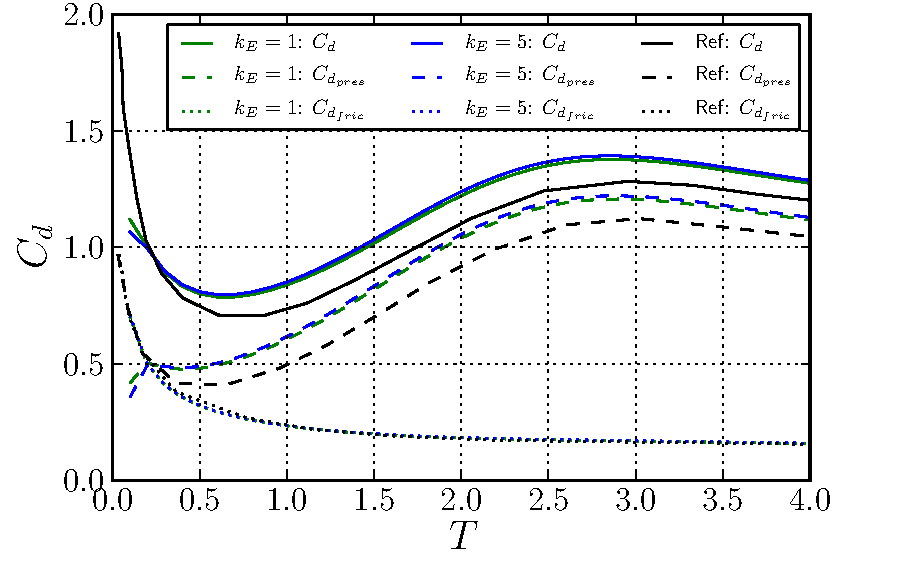
\includegraphics[width=\textwidth]{./figures/hybrid/isc/hybrid_ISC_drag_kComparison.pdf}
             \caption{Variation in Lagrangian time step size $\Delta t_L$: $k_E=1$ with $\Delta t_L = \Delta t_E$ and $k_E=5$ with $\Delta t_L = 5\cdot{\Delta t_E}$}
             \label{fig:hybrid_ISC_drag_kComparison}
     \end{subfigure}%
     ~ %add desired spacing between images, e. g. ~, \quad, \qquad etc.
       %(or a blank line to force the subfigure onto a new line)
     \begin{subfigure}[t]{0.49\textwidth}
             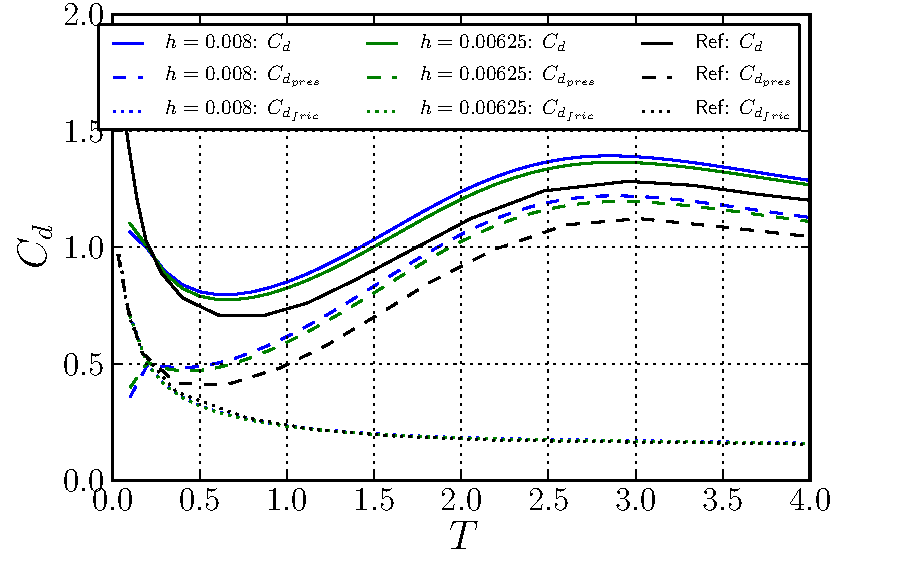
\includegraphics[width=\textwidth]{./figures/hybrid/isc/hybrid_ISC_drag_nBlobComparison.pdf}
             \caption{Variation in nominal blob spacing $h$: $h=0.008$ and $h=0.005$}
             \label{fig:hybrid_ISC_drag_nBlobComparison}
     \end{subfigure}
     
     \begin{subfigure}[b]{0.49\textwidth}
             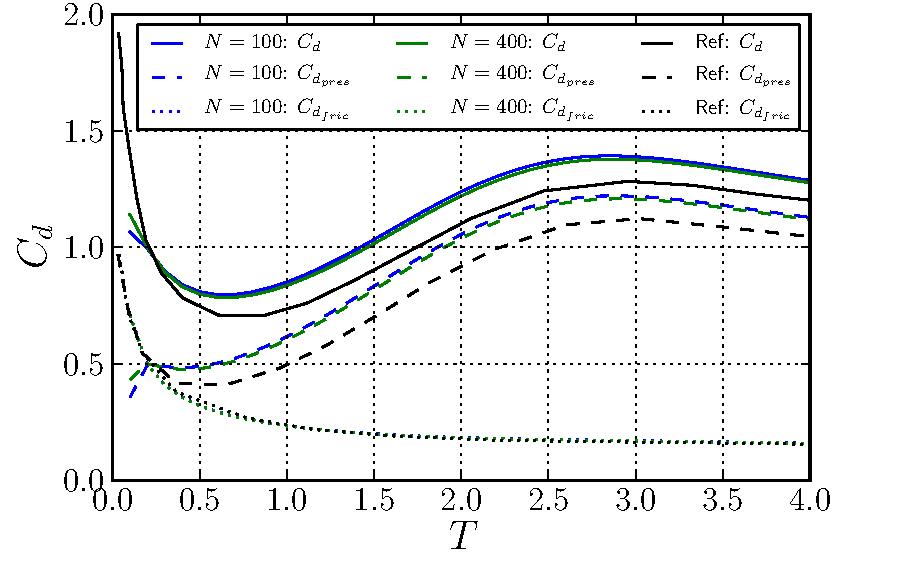
\includegraphics[width=\textwidth]{./figures/hybrid/isc/hybrid_ISC_drag_nPanelComparison.pdf}
             \caption{Variation in number of panels $N_{panels}$: $N=100$ and $N=400$}
             \label{fig:hybrid_ISC_drag_nPanelComparison}
	 \end{subfigure}
    
     \caption{Parameters sensitivity analysis on the drag evolution of the cylinder from $t=0$ to $t=4$, compared with literature data (\textbf{black}) obtained from Koumoutsakos and Leonard \cite{Koumoutsakos1995a}}
     \label{fig:hybrid_ISC_parameterSensitivity}
	\end{figure}

The second focus of the impulsively started cylinder is the long run, $t=0$ to $t=40$, evolution of the drag and lift of the cylinder. We performed similar comparison as done in section ??. An artificial perturbation was induced according to Leocointe \& Piquet \cite{Lecointe1984}. Figure \ref{fig:hybrid_cylinder_LongRun_liftDrag} shows the evolution of the lift coefficient $C_l$, and the drag coefficient $C_d$ of hybrid simulation, FE only simulation, and the reference data from RosenFeld et al. \cite{MosheRosenFeldDochanKwak1991}. 

	\begin{figure}[!p]
	\showthe\columnwidth
	\centering
	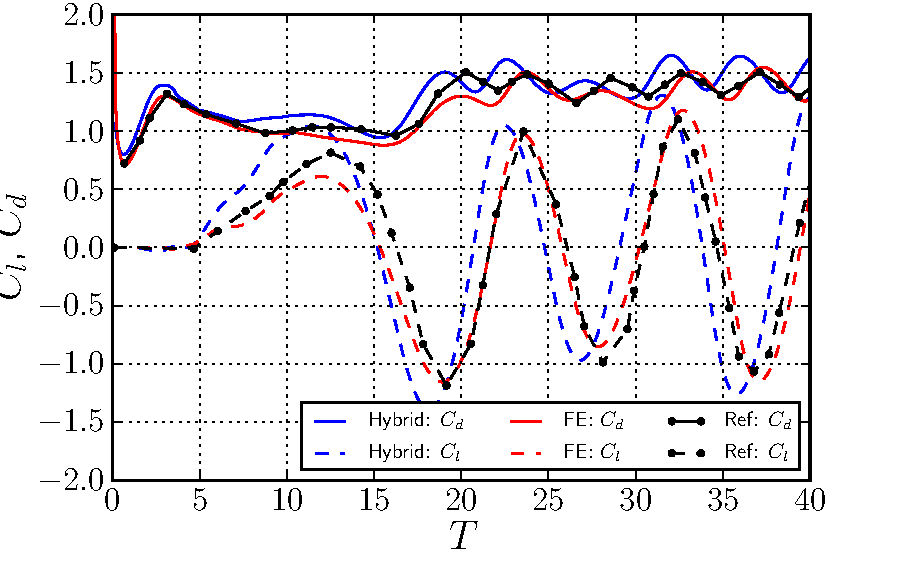
\includegraphics[width=0.6\linewidth]{./figures/hybrid/isc/hybrid_cylinder_LongRun_liftDrag.pdf}
	\caption{Evolution of the lift and drag coefficient from $t=0$ to $t=40$ with artificial perturbation \cite{Lecointe1984}. The figure compares hybrid ({\color{plotBlue}{\textbf{blue}}}), FE only ({\color{plotRed}{\textbf{red}}}), and the reference data (\textbf{black}) from RosenFeld et al. \cite{MosheRosenFeldDochanKwak1991}.}
	\label{fig:hybrid_cylinder_LongRun_liftDrag}
	\end{figure}

Investigating the evolution of drag shows that the hybrid simulation has higher drag. After $t=5$, there is slight mismatch in the oscillation of the drag. However observing the amplitude fluctuation, we see that the simulation tend to fluctuate around $C_d=1.4$. Observing the evolution of lift shows that the hybrid simulation has a larger initial amplitude. Furthermore, there exist a negative phase shift in the amplitude. However, at time progress, $t>20$, we see that the frequency and the amplitude of the oscillation is similar to the reference data.

Figure \ref{fig:hybrid_cylinder_LongRun_contourfComparison} compares the vorticity field of the hybrid simulation, and the FE only simulation at $t=[10,20,30,40]$. The shed vorticity of the hybrid simulation matches reasonably well with the FE only with a slight dif

	\begin{figure}[!p]
	\showthe\columnwidth
	\centering
	\includegraphics[width=\linewidth]{./figures/hybrid/isc/hybrid_cylinder_LongRun_contourfComparison_compressed-crop.png}
	\caption{hybrid cylinder LongRun contourfComparison}
	\label{fig:hybrid_cylinder_LongRun_contourfComparison}
	\end{figure}

	\begin{figure}[!p]
     \centering
     \begin{subfigure}[t]{0.49\textwidth}
             \includegraphics[width=\textwidth]{./figures/hybrid/isc/hybrid_isc_firstDipole_hybrid_compressed-crop.png}
             \caption{Hybrid}
             \label{fig:hybrid_isc_firstDipole_hybrid_compressed-crop}
     \end{subfigure}%
     ~ %add desired spacing between images, e. g. ~, \quad, \qquad etc.
       %(or a blank line to force the subfigure onto a new line)
     \begin{subfigure}[t]{0.49\textwidth}
             \includegraphics[width=\textwidth]{./figures/hybrid/isc/hybrid_isc_firstDipole_FE_compressed-crop.png}
             \caption{FE only}
             \label{fig:hybrid_isc_firstDipole_FE_compressed-crop}
     \end{subfigure}
     \caption{First dipole}
     \label{fig:hybrid_isc_firstDipole}
	\end{figure}

A through investigation of the oscillation requires a longer simulation where the amplitude of the oscillation would become fixed. However, due to the lack of computational resources, a longer simulation than $t=40$ with the current simulation parameters was not feasible.
	
	
	
\subsection{Conclusion}	


%In conclusion, we 
\section{Stalled Elliptic airfoil at $Re=5000$}

\subsection{Problem Definition}

The stalled airfoil performed similar to the impulsively started cylinder.

The parameters are tabulated below.

	\begin{figure}[!h]
	\showthe\columnwidth
	\centering
	%\includegraphics[trim=0cm 2.5cm 0cm 2.5cm, clip, width=\linewidth]
	\includegraphics[width=0.6\linewidth]{./figures/hybrid/ellipse/hellipticAirfoil_dd-crop.pdf}
	\caption{[\textit{Not to Scale}] }
	\label{fig:hellipticAirfoil_dd-crop}
	\end{figure}

\subsection{Results and Discussion}

	\begin{figure}[!p]
	\showthe\columnwidth
	\centering
	\includegraphics[width=\linewidth]{./figures/hybrid/ellipse/hybrid_ellipse_HybridvsFE_contourDeviation_compressed-crop.png}
	\caption{hybrid ellipse HybridvsFE contourDeviation}
	\label{fig:hybrid_ellipse_HybridvsFE_contourDeviation}
	\end{figure}

	\begin{figure}[!p]
	\showthe\columnwidth
	\centering
	\includegraphics[width=\linewidth]{./figures/hybrid/ellipse/hybrid_ellipse_Hybrid_contours_compressed-crop.png}
	\caption{hybrid ellipse Hybrid contours}
	\label{fig:hybrid_ellipse_Hybrid_contours}
	\end{figure}

	\begin{figure}[!p]
     \centering
     \begin{subfigure}[t]{0.49\textwidth}
             \includegraphics[width=\textwidth]{./figures/hybrid/ellipse/hybrid_ellipseForce_CL.pdf}
             \caption{Hybrid}
             \label{fig:hybrid_ellipseForce_CL}
     \end{subfigure}%
     ~ %add desired spacing between images, e. g. ~, \quad, \qquad etc.
       %(or a blank line to force the subfigure onto a new line)
     \begin{subfigure}[t]{0.49\textwidth}
             \includegraphics[width=\textwidth]{./figures/hybrid/ellipse/hybrid_ellipseForce_CD.pdf}
             \caption{FE only}
             \label{fig:hybrid_ellipseForce_CD}
     \end{subfigure}
     \caption{Forces}
     \label{fig:hybrid_ellipseForce}
	\end{figure}
	
	
	
	
%\section{Clercx-Bruneau dipole convection at $Re=625$}
%
%	\subsection{Comparison of vorticity contours}
%	
%	\subsection{Variation in maximum vorticity}
%	
%	\subsection{Variation in kinetic energy}
%	
%	\subsection{Variation in enstrophy}

%\section{Clercx-Bruneau dipole collision at $Re=625$}
%
%	\subsection{Comparison of vorticity contours}
%	
%	\subsection{Variation in maximum vorticity}
%	
%	\subsection{Variation in kinetic energy}
%	
%	\subsection{Variation in Enstrophy}
%	
%	\subsection{Variation in Palinstrophy}

%\section{Impulsively started cylinder problem at $Re=550$}
%
%	\subsection{Evolution of the wake}
%	
%	\subsection{Evolution of pressure and friction drag}
%	
%	\subsection{Evolution of lift}


%\section{Moving body}
%
%	\subsection{Error due to pertubation lag}
%
%\section{Proof of concepts}
%
%	\subsection{Multiple cylinder case}
%	
%	\subsection{Stalled airfoil at $Re=5000$}
%
%\section{Summary}